\documentclass[a4paper,10pt,twocolumn]{article}

\usepackage[T1]{fontenc}
\usepackage[utf8]{inputenc}
\usepackage[english]{babel}
\usepackage[sort&compress]{natbib}
% \setcitestyle{authoryear,open={((},close={))}}

\usepackage{amsmath}
\usepackage{amssymb}

\usepackage{xcolor}
\usepackage{graphicx, url}
\usepackage{grffile}

\graphicspath{{../assets/}}

\usepackage{subcaption}

\usepackage{booktabs}

\title{Bayesian Sparsification Methods for Deep Complex-valued Networks}
\author{Ivan Nazarov, and Evgeny Burnaev}

%% notation
\newcommand{\real}{\mathbb{R}}
\newcommand{\cplx}{\mathbb{C}}
\newcommand{\iu}{{\jmath}}
\newcommand{\tr}[1]{\mathop{tr}{#1}}

\newcommand{\hop}{{\mkern-1.5mu\dagger}}
\newcommand{\conj}[1]{\overline{#1}}

% \renewcommand{\top}{{\mkern-1.5mu\intercal}}
\renewcommand{\vec}[1]{\overrightarrow{#1}}
\newcommand{\diag}[1]{\mathrm{diag}{#1}}

%% drafting macro
\newcommand{\important}[1]{\textbf{\!\colorbox{red}{#1}\!}}
\newcommand{\attn}[2]{\textbf{\color{red} #2~\textsuperscript{\textit{[#1]}}}}
\newcommand{\verify}[1]{\textit{\!\colorbox{red}{#1}\!}}
\newcommand{\rewrite}[1]{\attn{rewrite}{#1}}
\newcommand{\todo}[1]{{\color{blue} [TODO]} \important{#1}}

%% red-highlight missing citations
\usepackage{etoolbox}
\makeatletter
\patchcmd{\@citex}{\bfseries ?}{\colorbox{red}{\bfseries ?}}{}{}
\makeatother

\begin{document}
\maketitle

\begin{abstract}
With continual miniaturization ever more applications of deep learning can be found
in embedded systems, where it is common to encounter data with natural complex domain
representation. To this end we extend Sparse Variational Dropout to complex-valued neural
networks and verify the proposed Bayesian technique by conducting a large numerical
study of the performance-compression trade-off of $\cplx$-valued networks on two tasks:
image recognition on MNIST-like and CIFAR10 datasets and music transcription on MusicNet.
We replicate the state-of-the-art result by \citet{trabelsi_deep_2018} on MusicNet with
a complex-valued network compressed by $50-100\times$ at a small performance penalty.
\end{abstract}

\section{Introduction} % (fold)
\label{sec:introduction}

% general intro text with motivation
Deep neural networks are an integral part of machine learning and data science toolset
for practical data-driven problem solving. With continual miniaturization ever more
applications can be found in embedded systems. Common embedded applications include
on-device image recognition and signal processing. Despite recent advances in generalization
and optimization theory specific to deep networks, deploying in actual embedded hardware
remains a challenge due to storage, real-time throughput, and arithmetic complexity
restrictions \citep{he_amc:_2018}. Therefore, compression methods for achieving high
model sparsity and numerical efficiency without losing much in performance are especially
relevant.
% Solving the storage and artihmetic constraints encourages development of model compression
% and sparsification methods, that focus on favourable trade-off between performance and size.

% applications of cvnn
Complex-valued nature of the data in acoustic and radio signal processing has been
the main driver behind the adoption of $\cplx$-valued neural networks ($\cplx$VNN).
\citet{hirose_complex-valued_2009} argues that the combined phase-magnitude effect of
$\cplx$-valued transformations reduces removes the excess degrees of freedom, that cause
degenerate transformation in $\real$-valued networks with twice the feature dimensions.
Their study demonstrates superiority of $\cplx$VNN in landmine detection using ground
penetrating radar imaging. Other examples, where $\cplx$-valued networks have outperformed
$\real$-valued networks include magnetic resonance \citep{hui_mri_1995,wang_deepcomplexmri_2020}
and radar imaging \citep{haensch_complex-valued_2010,zhang_complex-valued_2017}, music
transcription and spectral speech modelling \citep{wisdom_full-capacity_2016,trabelsi_deep_2018},
and wireless signal classification \citep{yang_complex_2019}. \citet{tarver_design_2019}
have lowered the out-of-band power leakage with a $\cplx$-valued network for digital
signal predistortion. The networks have also been applied to non $\cplx$-valued domains,
such as image classification \citep{popa_complex-valued_2017}, sequence modelling
\citep{danihelka_associative_2016}, and motion prediction \citep{wolter_complex_2018},
and for stabilizing back-propagation in RNN \citep{wisdom_full-capacity_2016}.

% motivation and other methods
Despite promising results for embedded signal processing applications, $\cplx$-valued
networks remain a niche in deep learning, and as such little attention has been paid
to compression methods specific to $\cplx$VNN. \citet{wu_compressing_2019} adapt $k$-means
quantization to $\cplx \simeq \real^2$ parameters and successfully compress $\cplx$VNN
with the ``prune-quantize-code'' procedure of \citet{han_deep_2016}.

Yet there is an abundance of research related to real-valued network compression, and
many results can be applied to $\cplx$VNN. Methods such as knowledge distillation
\citep{hinton_distilling_2015}, which trains a small network to replicate a large
well-trained teacher, low-rank matrix \citep{denton_exploiting_2014} and tensor decomposition
\citep{novikov_tensorizing_2015}, or magnitude-based parameter pruning \citep{zhu_prune_2018}
can be adapted to $\cplx$VNN without modifications. Parameter quantization and conversion
from floating to fixed point arithmetic \citep{courbariaux_training_2015,uhlich_mixed_2020},
appear to be readily applicable as well. \citet{louizos_learning_2018} propose probabilistic
$\ell_0$ regularization through multiplicative $[0, 1]$-valued stochastic masks with
distribution having an atom at $0$, yet differentiable via the reparameterization trick
\citep{kingma_auto-encoding_2014}. By sharing a single mask value within a group of
parameters their approach can be adapted to $\cplx$ parameters. However, methods such
as Hessian-based parameter pruning \citep{lecun_optimal_1990} or Sparse Variational Dropout
\citep{molchanov_variational_2017} require additional considerations.
% the more explicitly zero parameters there is, the less computations is needed.

% segue into why we chose sparse VD rather than anything else
% (sparsity tech large-scale models) gale-elsen-hooker.tex
\citet{gale_state_2019} compare magnitude pruning, $\ell_0$ regularization and Sparse
Variational Dropout (VD) on large-scale models. Their results suggest that VD may achieve
good accuracy-sparsity balance and outperform pruning and $\ell_0$ in deep architectures,
although pruning is preferred for simplicity, stability and speed. They also observe that
VD induces non-uniform sparsity throughout the model, which \citet{he_amc:_2018} have shown
to be essential for superior compression.
% Magnitude pruning induces user-specified sparsity distributions.

% our contribution
Sparse Variational Dropout is a Bayesian Variational Inference method with automatic
parameter relevance determination effect. In this study we extend \emph{Sparse VD} to
$\cplx$VNN, inspired by the results of \citet{gale_state_2019}, and motivated by seldom
application of Bayesian Inference to $\cplx$-valued networks \citep{popa_complex-valued_2018}
and apparent scarcity of compression methods specific to them. We assess the performance-%
compression trade-off of the extension by conducting a large-scale numerical study on
image classification on MNIST-like and CIFAR10 datasets and music transcription on MusicNet.
%
% THIS SHOULD GO TO CONCLUSIONS!
%
% L0 and dropout work in the low-to-mid sparsity range, variational dropout consistently
% ranked behind L0 on Transformer, and was bested by magnitude pruning for sparsity
% levels of 80\% and up. Variational dropout consistently produces models on-par or better
% than magnitude pruning on ResNet-50, and l0 fails to produce sparse models at all.
We expect the overall conclusion of \citet{gale_state_2019} to carry over to $\cplx$VNN,
since there is nothing fundamentally different in $\cplx$-valued versions of the methods
they study, except for the need to operate on pairs of parameters.

The paper is structured as follows. Sec.~\ref{sec:variational_dropout} reviews Variational
Dropout, and sec.~\ref{sec:c_valued_networks} provides a brief summary of the inner
working of complex-valued networks. The main contribution of this study is presented in
sec.~\ref{sec:c_variational_dropout}, where we outline the details of different variational
approximations and priors and derive the penalty terms in the evidence lower bound.
In sec.~\ref{sec:experiments} we evaluate the sparsification rate, compare the resulting
performance of various $\cplx$-networks proposed in prior work, and discuss the outcomes.


% section introduction (end)

\section{Variational Dropout} % (fold)
\label{sec:variational_dropout}

\subsection{Variational Inference} % (fold)
\label{sub:variational_inference}

% overview
In broad terms Bayesian Inference is a principled framework of reasoning about uncertainty
and a tool to update prior beliefs about model's parameters in accordance with evidence
or empirical data into a posterior distribution. The posterior is useful for inference
regarding unobserved data, predictive statistics, parameter confidence regions, and
model's uncertainty.
% intuitive definition of  of model given data is the same as probability of data under hypothesis (model)
% KL-div min & VI -- \citep{jordan_introduction_1999} approximate Bayesian inference
% SVI -- \citep{hoffman_stochastic_2013} scalable stochastic variant
% SGVB -- \citep{kingma_auto-encoding_2014} differentiable MCMC estimator of the evidence lower bound for SVI

For an observed dataset $
  D = (x_i)_{i=1}^N
$ and statistical model $
  p(D \mid \omega)
    = \prod_i \log p(x_i \mid \omega)
    % $D$ conditional independence given parameters $\omega$
$ with parameters $\omega$ the Bayes rule transforms prior hypotheses $\pi(\omega)$
about the unknown distribution of model's parameters into the posterior distribution: $
  p(\omega \mid D) = \tfrac{p(D \mid \omega) \pi(\omega)}{p(D)}
$.
%
% In general the marginal likelihood of the dataset is intractable $
%   p(D) = \mathbb{E}_{\pi(\omega)} p(D \mid \omega)
% $.
Save for the relatively simple set-ups, either the posterior distribution itself or the
mathematical expectations it is involved in are analytically intractable or impractical
to compute numerically. Variational Inference (VI), proposed by \citet{jordan_introduction_1999},
can be used in such cases to make approximate inference. The approach finds an approximation
within some distribution family $q_\theta(\omega)$, which is closest to the true posterior
distribution in terms of Kullback-Leibler divergence: $
  KL(q_\theta(\omega) \| p(\omega \mid D))
    % = \int \frac{dQ}{dP} \log{\frac{dQ}{dP}} P(d\omega)
    % = \int \frac{q(\omega)}{p(\omega)} \log{\frac{q(\omega)}{p(\omega)}} p(\omega) d\omega
    % = \mathbb{E}_{\omega \sim q}
    %   \log\frac{q(\omega)}{p(\omega)}
    = \mathbb{E}_{\omega \sim q_\theta}
      \log \tfrac{q_\theta(\omega)}{p(\omega \mid D)}
$. % The approximation family is chosen so that the expectations become tractable.
%
\citet{jordan_introduction_1999} show that this problem is equivalent to variational
\emph{maximization} of the \emph{Evidence Lower Bound} (ELBO)
\begin{equation}  \label{eq:elbo_general}
  \mathcal{L}(\theta; \lambda)
    = - KL(q_{\theta} \| \pi_{\lambda})
      + \sum_{i=1}^N \mathbb{E}_{\omega \sim q_{\theta}}
        \log p(x_i \mid \omega)
      % \mathbb{E}_{\omega \sim q_{\theta}}
        % \log\frac{q_\theta(\omega)}{\pi_{\lambda}(\omega)}
  % = \mathbb{E}_{\omega \sim q_{\theta}}
  %     \log{p_{\phi}(D \mid \omega) \pi_{\lambda}(\omega)}
  %   + \mathbb{H}(q_{\theta})
  \,,
\end{equation}
where the variational parameters $\theta$ and $\lambda$ parameterize the approximation
and the prior, respectively.
%
Kullback-Leibler and, by proxy, ELBO are standard objectives in VI, however it is possible
to use other objectives, provided the true posterior $p(\omega \mid D)$ is evaluated only
through $\log p(D \mid \omega)$ and $\log \pi(\omega)$, \citep{ranganath_operator_2018}.

% speed, scale, variance, family of suitable Var approximations
In subsequent years several improvements to Variational Inference approach were introduced.
To make VI able to handle large-scale datasets \citet{hoffman_stochastic_2013} proposed
\emph{Stochastic Variational Inference}, which uses stochastic gradient optimization of
\eqref{eq:elbo_general} based on inexpensive noisy unbiased gradient estimates of ELBO
computed on random mini-batches from the dataset. \citet{titsias_doubly_2014} translated
dependence on $\theta$ from $q_{\theta}$ to the functions inside the expectations of ELBO
and propose \emph{Doubly Stochastic Variational Inference}, which computes unbiased gradient
estimator based on both dataset subsampling and random draws from variational distribution
$q_{\theta}$. Note, that the KL divergence term can replaced by its unbiased differentiable
finite-sample estimator without forfeiting convergence of (doubly) SVI.

% The variance of the stochastic gradient directly affects convergence of SVI. 
Independently, \citet{kingma_auto-encoding_2014} proposed \emph{Stochastic Gradient
Variational Bayes}, which is an alternative efficient doubly stochastic estimator
applicable to models with parameters $\omega$ that are continuous random variables
amenable to the \emph{reparameterization trick}, i.e. $
  \omega \sim q_{\theta}(\omega)
$ is equivalent in distribution to $
  \omega = g_{\theta}(\varepsilon)
$ for some non-parametric random variable $
  \varepsilon \sim p(\varepsilon)
$ and $
  g(\varepsilon; \theta)
$ differentiable with respect to $\theta$. The estimator of \eqref{eq:elbo_general}
for $L$ reparameterized draws per datapoint in mini-batch of size $M$, is given by
\begin{equation}  \label{eq:sgvb_estimator}
  \widetilde{\mathcal{L}}(\theta; \lambda)
    = - KL(q_{\theta} \| \pi_{\lambda})
      % + \frac{N}{\lvert B \rvert} \sum_{i\in B}
        % \log p(x_i \mid \omega_i)b
      + \frac{N}{M L} \sum_{k,l}
        \log p(x_{i_k} \mid g(\varepsilon_{lk}; \theta))
      % + \frac{N}{M L} \sum_{k=1}^M \sum_{l=1}^L
      %   \log p(x_{i_k} \mid g(\varepsilon_{lk}; \theta))
        % \log p(D \mid \omega_{l})
        %   \Big\vert_{\omega_{l} = g(\varepsilon_{l}; \theta)}
      % =
      % - KL(q_{\theta} \| \pi)
      % + N \mathbb{E}_{B \sim \{D\}_M \otimes q_\theta^M}
        % \hat{\mathbb{E}}_{x,\omega \sim B}
          % \log p(x \mid \omega)
    \,,
\end{equation}
where $(x_{i_k})_{k=1}^M$ is a random mini-batch from $D$ and $
  (\varepsilon_{lk})_{l=1}^L
$ are $M$ independent iid samples from $p_\varepsilon$. \citet{figurnov_implicit_2019}
extended the scope of the reparameterization gradients to include continuous distributions
such as Gamma and von Mises. To handle the case of non-reparameterizable $\omega$ in
doubly stochastic VI, e.g. discrete random parameters, \citet{titsias_local_2015} proposed
\emph{local expectation gradients}, which is a version of REINFORCE gradient estimator
\citep{williams_simple_1992} with variance reduced by careful use of dependence
structures in the model.
% (reparameterization trick, pathwise gradient) $q_{\theta}(d\omega)$ is a push-forward
% of $p(d\varepsilon)$ by a differentiable map $g(\varepsilon; \theta)$.
% % http://stillbreeze.github.io/REINFORCE-vs-Reparameterization-trick/#fn:1
% rao-blackwellization (http://pyro.ai/examples/svi_part_iii.html)

% The Local Reparameterization Trick reduces the variance of SGVB
% even further by sampling independent weight matrices for
% each data-point inside mini-batch. So we need both original SGVB
% (per sample randomness) and local reparameterization (that is an
% efficient and less noisy equivalent to per-sample weight sampling)
% SGVB is specifically for VAE (local latent variables per data-point)
% what Kingma propose is SGVB for global shared latent variables aka
% WEIGHTS!!
In this study we use the SGVB estimator \eqref{eq:sgvb_estimator} with $L=1$ and the
\emph{local reparameterization trick} proposed by \citet{kingma_variational_2015}. They
argued that this gradient estimator can be made more statistically and computationally
efficient, if the structure of the model permits translating global stochasticity of
$\omega$ down to local intermediate states of computation.
%
The class of models that are allow this include non-recurrent computational graphs,
exemplified by neural networks with parameters $\omega \sim q_\theta$. In this case
\eqref{eq:sgvb_estimator} would require that the \emph{entire} set of network's parameters
$\omega$ be independently drawn for each element in the mini-batch. However, noting
that the parameters in a network naturally decompose into subsets with non-overlapping
layer-wise effects, it is standard to assume that the approximation $
  q_\theta(\omega)
$ is factorized over layers. Furthermore, if $
  % \omega =
  W \in \mathbb{R}^{n\times m}
$ in a linear layer $
  y = b + W^\top x
$ with $
  q_\theta(W)
    = \prod_{ij}
      \mathcal{N}(w_{ij} \vert\, \mu_{ij}, \sigma_{ij}^2)
$, then by virtue of $y$ being a linear transformation of $W$, we get
\begin{equation}  \label{eq:r-gauss-trick}
  q(y) = \prod_i \mathcal{N}\Bigl(
        y_i \big\vert\,
        b_i + \sum_j \mu_{ij} x_j,
        \sum_j \sigma^2_{ij} x_j^2
    \Bigr)
  \,.
\end{equation}
This yields outputs equivalent in distribution to sampling $W$ for each element in
the mini-batch, which produces the SGVB estimator with smaller variance, as demonstrated
by \citet{kingma_variational_2015}.
% Similar idea to \eqref{eq:r-gauss-trick} was proposed by \citet{wang_fast_2013} to speed
% up Gaussian dropout.

% subsection variational_inference (end)

\subsection{Dropout} % (fold)
\label{sub:dropout}

With a special posterior approximation family $q_\theta$ and suitable prior $\pi$,
Variational Inference can be used as model regularization and sparsification technique.

% on dropout
Dropout, proposed by \citet{hinton_improving_2012}, prevents overfitting by injecting
multiplicative binary noise into layer's weights, which breaks up co-adaptations that
could occur during training. \citet{wang_fast_2013} argued that the overall effect of
binary dropout on the intermediate outputs can be approximated by a Gaussian with weight-input
dependent mean and variance via the Central Limit Theorem. \citet{srivastava_dropout:_2014}
proposed using independent $\mathcal{N}(1, 1)$ multiplicative noise, arguing that higher
entropy of a Gaussian has better regularizing effect. \citet{gal_dropout_2016} showed
that Dropout is a Bayesian approximation method with close ties to deep Gaussian Processes
that yields inexpensive model uncertainty estimates. In a study concerning multitask learning
\citet{cheung_superposition_2019} demonstrated the possibility of storing task-specific
parameters in non-destructive superposition within a single network. Regarding Dropout
their argument implies that if the single task setting is viewed as multitask learning
with replicated task, then by sampling uncorrelated binary masks Dropout acts as a
superposition method, utilizing the learning capacity of the network better.
% many identical copies of the same task; \cite[Appendix A.1]{cheung_superposition_2019}
% (fast dropout gauss-approx) wang-manning.tex
% (gauss dropout) srivastava-et-al.tex

% VD is a Bayesian perspective on dropout regularization \citep{hinton_improving_2012} offered
% by \citet{kingma_variational_2015} and repurposed for sparsification by \citet{molchanov_variational_2017}.
%
\citet{kingma_variational_2015} provided a unifying perspective on Dropout, DropConnect
\citep{wan_regularization_2013}, and Gaussian dropout \citep{wang_fast_2013} through
the lens of Variational Inference methods and propose \emph{Variational Dropout}. They
argued that the multiplicative noise introduced by Dropout methods induces a distribution
equivalent to a fully factorized variational posterior of the form $
  q_\theta(\omega) = \prod_j q_{\theta}(\omega_j)
$, where $q_{\theta}(\omega_j)$ is $\omega_j = \mu_j \xi_j$ with $
  \xi_j \sim p_\theta(\xi_j)
$ iid from some $p_\theta(\xi)$.
%
% Binary dropout with rate $p \in (0, 1)$ uses $
%   p_\xi
%     = \mathcal{B}\bigl(
%       \{0, \tfrac1{1-p}\}, 1-p
%     \bigr)
% $, whereas in Gaussian dropout $
%   \xi \sim \mathcal{N}(1, \alpha)
% $ for $\alpha = \tfrac{p}{1-p}$.
% This suggests making $\alpha$ a variational parameter
% and optimizing it in \eqref{eq:elbo_general} with an appropriate penalty term. Thus,

Variational Dropout uses \emph{fully factorized Gaussian} approximation $
  q_\theta(\omega)
    = \prod_j \mathcal{N}(\omega_j \vert\, \mu_j, \alpha_j \mu_j^2)
$ and factorized scale invariant log-uniform prior $\pi(\omega)$ with $
  \pi(\omega_j) \propto \lvert \omega_j \rvert^{-1}
$. \citet{molchanov_variational_2017} noticed that $\alpha_j$ reflect the relevance of the
parameter $\omega_j$ it is associated to by being the ratio of its squared mean to its
effective variance. Based on this observation they proposed \emph{Sparse Variational Dropout},
a modification that enables automatic model sparsification by optimizing $\alpha_j$ for each
individual parameter. \citet{louizos_bayesian_2017} extended the idea to structured sparsity
by considering hierarchical prior and variational approximation. They grouped the parameters
$\omega_j$ and coupled them within each one through a shared latent variable, which on the
whole enabled pruning entire input features in each layer.
% {louizos_bayesian_2017} eq. (11) variance -> gaussian entropy -> informative bits
%

Simultaneously \citet{molchanov_variational_2017} proposed to use \emph{Additive Noise
Parameterization} in the factorized Gaussian $q_\theta(\omega)$ in conjunction with the
Local Reparameterization Trick. They reverted the $(\mu, \alpha)$ parameterization in
$q_\theta(\omega)$ back to $(\mu, \sigma^2)$, arguing that it reduces the variance of the
SGVB \eqref{eq:sgvb_estimator}, by rendering the gradient with respect to $\mu$ independent
from the local noise, injected by \eqref{eq:r-gauss-trick}. This modification is important
for pruning, since $\mu$ of relevant parameters are used as estimates of their values.

Due factorization assumption, the term $KL(q_\theta \| \pi)$ in \eqref{eq:sgvb_estimator}
for Sparse VD unravels into $
  \sum_j K(\tfrac{\sigma^2_{j}}{\mu_{j}^2})
$ with
\begin{equation}  \label{eq:improper-kl-div-real}
  K(\alpha)
    \propto \frac12 \mathbb{E}_{\varepsilon \sim \mathcal{N}(0, 1)}
        \log{\Bigl\lvert \tfrac1{\sqrt{\alpha}} + \varepsilon \Bigr\rvert^2}
      % \frac12 \mathbb{E}_{\varepsilon \sim \mathcal{N}(0, 1)}
      %   \log{\bigl\lvert 1 + \sqrt{\alpha} \varepsilon \bigr\rvert^2}
      % - \frac12 \log{\alpha}
  \,.
\end{equation}
\citet{kingma_variational_2015} approximated $K(\alpha)$ over $\alpha \in (0, 1)$ by
a non-linear polynomial, and later \citet{molchanov_variational_2017} refined the
approximation of \eqref{eq:improper-kl-div-real} by a nonlinear regression based on
sigmoid and soft-plus.
% see p.6 sec 3.4 of kingma_variational_2015
In appendix~\ref{sec:real-chisq-grad} we verify the value and the derivative of their
approximation against the Monte-Carlo estimate of \eqref{eq:improper-kl-div-real} for
$\alpha$ varying over a fine logarithmic grid and the gradient of \eqref{eq:improper-kl-div-real},
for which we obtain an exact expression.
% (!) good for SGVB: gradient-based methods require unbiased gradient estimates
% (in) it is in poor taste to brag about this beign the first time anyone has derived a
% derivative of an intractable function.

\citet{kharitonov_variational_2018} addressed theoretical issues with improper prior
$\pi$ in Sparse VD, emphasized by \citet{hron_variational_2018}, and proposed
\emph{Automatic Relevance Determination} Variational Dropout, by replacing $\pi(\omega_j)$
with a proper Gaussian prior $
  \pi_\lambda(\omega_j) = \mathcal{N}(\omega_j \vert\, 0, \tau_j^{-1})
$ with learnable precision $\tau_j > 0$ \citep{neal_bayesian_1996}. This recast the VD
as the \emph{Empirical Bayes} approach, which performs Bayesian Inference over $\omega$,
but uses Maximum Likelihood estimates for the hyper-parameters $\lambda$,
\citep{mackay_bayesian_1994}. Maximizing \eqref{eq:sgvb_estimator} over $\tau$, holding
other parameters fixed, yields $
  \tau^*_j = {(\mu_j^2 + \sigma^2_j)}^{-1}
$, whence
\begin{equation}  \label{eq:ard-kl-div-real}
  K(\alpha)
    = \frac12 \sum_j \log{\bigl(1 + \tfrac1{\alpha} \bigr)}
    \,.
\end{equation}
% \begin{align}
%   \pi(\omega)
%     &
%     = \prod_J \pi(s_J)
%       \prod_{j\in J} \pi(\omega_j \vert s_J)
%     \propto \prod_J \frac1{\lvert s_J \rvert}
%       \prod_{j\in J} \mathcal{N}(\omega_j \vert 0, s_J^2)
%     \,, \\
%   q_\theta(\omega)
%     &
%     % = \prod_J q_\theta(s_J)
%     %   \prod_{j\in J} q_\theta(\omega_j \vert s_J)
%     = \prod_J \mathcal{N}(s_J \vert \mu_J, \alpha_J \mu_J^2)
%       \prod_{j\in J} \mathcal{N}(\omega_j \vert \mu_j s_J, \sigma_j^2 s_J^2)
%     \,.
% \end{align}

% practical difference between them?

% subsection dropout (end)

% section variational_dropout (end)


\section{$\cplx$-valued networks} % (fold)
\label{sec:c_valued_networks}

% implementation
$\cplx$-valued neural networks are networks that rely on the arithmetic in the complex
domain. To achieve this implementations of $\cplx$VNN use the geometric (planar) representation
of a complex number as paired \emph{real} and \emph{imaginary} values, $\cplx \simeq \real^2$,
ensuring that the resulting $\real$-valued computational graph respects $\cplx$-arithmetic.
For example, $
  f\colon \cplx^n \to \cplx^m
$ is identified with a real vector-valued function $
  F\colon \real^{2 m} \to \real^{2 m}
$ defined via $
  F(u, v) = (\Re f(u + \iu v), \Im f(u + \iu v))
$, $\Re$ and $\Im$ denoting the real and imaginary parts, respectively. When $f$ is
a $\cplx$-valued linear transformation, the computations are ``wired'' so that
\begin{equation}  \label{eq:cplx-lin-op}
  % F\colon
  %   (u, v)
  %     \mapsto \Bigl(
  %       P u - Q v,
  %       P v + Q u
  %     \Bigr)
  F(u, v)
    =
    \begin{pmatrix}
      P u - Q v \\
      P v + Q u
    \end{pmatrix}
    = \begin{pmatrix}
      P & - Q \\ Q & P
    \end{pmatrix} \begin{pmatrix}
      u \\ v
    \end{pmatrix}
    \,,
\end{equation}
with $
  P, Q \colon \real^{n} \to \real^{m}
$ given by $P = \Re f$ and $Q = \Im f$ restricted to $\real^{n}$.
% The downside is that, for instance, one $\cplx$-valued convolution requires up to
% four $\real$-valued convolution operations.
%
Nonlinearities in $\cplx$VNN can be hyperbolic functions or maps that operate on
$\cplx$ numbers in planar form, $
  z \mapsto \sigma(\Re{z}) + \iu \sigma(\Im{z}) % split
$, or polar form $
  % z \mapsto \sigma(\lvert z\rvert, \arg{\!(z)})
  r e^{\iu \phi} \mapsto \sigma(r, \phi)
$.
% \citep{savitha_2011,hirose_generalization_2012,arjovsky_unitary_2016,guberman_complex_2016}

This $\cplx \simeq \real^2$ identification allows straightforward retrofitting of $\cplx$VNN
into existing $\real$-valued auto-differentiation frameworks for deep learning. This
act is backed by Wirtinger ($\cplx\real$) calculus, which enables generalized treatment
of functions of complex argument, by regarding $z$ and $\conj{z}$ as independent variables
and defining derivatives with respect to them through partial derivatives with respect
to real and imaginary parts of each argument. These definitions simplify manual calculations
of $\cplx$ derivatives and satisfy the product and chain rules, respect complex conjugation
and linearity for $\cplx \to \cplx$ maps. $\cplx\real$ calculus was used to define $\cplx$
version of back-propagation, \citep{benvenuto_complex_1992,guberman_complex_2016}. However,
since auto-differentiation frameworks can algorithmically handle computational graphs
of arbitrary complexity, explicit use of Wirtinger derivatives is not required, especially
considering the fact that the direction of the steepest ascent of a $\cplx\to \real$
function is given by complex conjugate gradient $\nabla_{\conj{z}}$, which coincides
with the classical gradient of the same function viewed as $\real^2 \to \real$,
(see appendix~\ref{sub:wirtinger_calculus}).
%
% in natively $\cplx$-valued backprop it would be necessary to modify the existing sgd
% to explicitly use $\nabla_{\conj{z}} f(z)$, while no such modification is necessary
% in re-im. If some inner activation of a $\cplx$VNN is holomorphic, i.e. satisfies
% Cauchy-Riemann conditions, then that particular step of in the chain rule that is
% backprop can be simplified by assuming one piece of the tracked gradient to be exact
% zero. But other wise it is necessary to track both $\partial_{\conj{z}}$ and $\partial_{z}$.
%
% Training a $\cplx$VNN involves optimizing a real-valued objective with respect to
% complex valued arguments.
%
% The computed gradients are theoretically justified
% - CR dictates the it is necessary to track both $z$ and $\conj{z}$ derivatives
% - the direction of largest increase in f: C-R is given by the gradient with
% respect to the conjugate, which coincides in the re-im representation with 
% the ordinary gradient wrt u and v
% - the Chain Rule in CR holds and when a holomorphic C-C function is backproped
% the autodiff just wastes cycles on computing its conj-derivative (rather than assuming
% it to be zero)

% Although $\cplx$-valued dense layers and back-propagation have been around since early
% 1990-s, one of the earliest accounts
Development of deep $\cplx$-valued networks has been active. \citet{haensch_complex-valued_2010}
put forward $\cplx$-valued convolutional networks, \citet{guberman_complex_2016} and
\citet{popa_complex-valued_2017} developed modifications of pooling, \citet{arjovsky_unitary_2016}
and \citet{wisdom_full-capacity_2016} proposed $\cplx$-valued RNNs with unitary recurrent
transition matrices, and \citet{danihelka_associative_2016} developed $\cplx$-valued
holographic representations for LSTMs. More recently \citet{trabelsi_deep_2018} proposed
$\cplx$-valued batch-normalization and weight initialization, \citet{wolter_complex_2018}
investigated different $\cplx$-valued gating mechanisms for RNNs, \citet{yang_complex_2019}
proposed $\cplx$-valued self-attention and complex transformer architecture. It merits
noting that \citet{gaudet_deep_2018} generalized $\cplx$VNN further to deep quaternion-valued
networks, and \citet{vecchi_compressing_2020} studied sparsity inducing regularizers for
them.
% complex-valued distributions \citep{pav_moments_2015,taubock_complex-valued_2012},
% and \citep{karseras_caution:_2014}

% This is too abrupt: first intro into what Cplx- valued nets are, then the representation 
% and how it dictates the architecture, and ultimately bioils down to representation
% u(x, y) + j v(x, y) as a R2->R2 map.

% \todo{read on holomorphic nets}

% section c_valued_networks (end)


\section{$\cplx$-Variational Dropout} % (fold)
\label{sec:c_variational_dropout}

We propose to use fully factorized complex Gaussian posterior approximation and $\cplx$
variant of the local reparameterization trick to extend Bayesian Dropout techniques to
$\cplx$-valued networks. In this section we describe the approximation and derive the
divergence penalties in \eqref{eq:sgvb_estimator}. Similarly to $\real$-valued Variational Dropout,
the proposed $\cplx$-valued extension can be straightforwardly enhanced to provide
structured sparsity.


\subsection{$\cplx$-Gaussian Distribution} % (fold)
\label{sub:c_gauss_and_local_rep}

A vector $z\in \cplx^m$ has complex Gaussian distribution, $
  q(z) = \mathcal{N}^{\cplx}_m(\mu, \Gamma, C)
$ with mean $\mu \in \cplx^m$ and $\cplx^{m\times m}$ covariance and relation matrices
$\Gamma$ and $C$, respectively, if
\begin{equation}  \label{eq:cn-paired-real-density}
  \begin{pmatrix}
    \Re z \\ \Im z
  \end{pmatrix}
    \sim \mathcal{N}_{2 m}\biggl(
      \Bigl(
        \begin{smallmatrix}
          \Re \mu \\ \Im \mu
        \end{smallmatrix}
      \Bigr),
      \tfrac12 \Bigl(
        \begin{smallmatrix}
          \Re{(\Gamma + C)} & \Im{(C - \Gamma)} \\
          \Im{(\Gamma + C)} & \Re{(\Gamma - C)}
        \end{smallmatrix}
      \Bigr)
    \biggr)
    \,,
\end{equation}
provided $\Gamma \succeq 0$, $\Gamma^{\hop} = \Gamma$, $C^\top = C$, and $
  \conj{\Gamma} \succeq C^{\hop} \Gamma^{-1} C
$.
% notation
Here, $M^{\top}$ is the matrix transpose, $\conj{M}$ is elementwise complex
conjugation, and $M^{\hop} = (\conj{M})^\top$ denotes Hermitian conjugate.
%
Matrices $\Gamma$ and $C$ are given by $
  \mathbb{E} (z - \mu)(z - \mu)^{\hop}
$ and $
  \mathbb{E} (z - \mu)(z - \mu)^{\top}
$, respectively, and $z$ is a \emph{proper} $\cplx$-Gaussian vector if $z$ and
$\conj{z}$ are uncorrelated, i.e. $C = 0$.
%
The entropy of $z$ terms of $\Gamma$ and $C$ is
\begin{align}
  \mathbb{H}(q)
    & = - \mathbb{E}_{z \sim q} \log{q(z)}
    \notag \\
    % &
    % entropy of \mathcal{N}_n(\mu, \Sigma)
    %   % = \tfrac12 \log \det{(2 \pi \Sigma)}
    %   % + \tfrac12 \mathop{tr}{(
    %   %     \Sigma^{-1}
    %   %     \mathbb{E}_{x\sim q(x)}
    %   %       (x - \mu) (x - \mu)^\top
    %   %   )}
    %   = \tfrac12 \log \det{(2 \pi e \Sigma)}
    % = \tfrac12 \log \det{\biggl(
    %   2 \pi e \tfrac12
    %   \begin{pmatrix}
    %     \Re{(\Gamma + C)} & - \Im{(\Gamma - C)} \\
    %     \Im{(\Gamma + C)} &   \Re{(\Gamma - C)}
    %   \end{pmatrix}
    % \biggr)}
    % \notag \\
    % &
    % = \begin{bmatrix}
    %   r_1 + j r_2 \to r_1 \\  % sufficient for C=0 case
    %   j r_1 + r_2 \to r_2     % j conj of transformation for r1, det x 2
    % \end{bmatrix}
    % = \tfrac12 \log \det{\biggl(
    %   % \det{[I & j I \\ j I & I]} = \det{I} \det{I - jI I^{-1} jI} = \det{2 I}
    %   % left apply : thus dividing by \sqrt{2}
    %   \tfrac1{\sqrt{2}} 2 \pi e \tfrac12
    %   \begin{pmatrix}
    %     \Gamma + C & j (\Gamma - C) \\
    %     j (\conj{\Gamma} + \conj{C}) & \conj{\Gamma} - \conj{C}
    %   \end{pmatrix}
    % \biggr)}
      % % Implicitly using the fact that for a non-singular $\Omega$ we have $
      % %   \det{A}
      % %     = \tfrac{\det{(\Omega A)}}{\det{\Omega}}
      % %     = \tfrac{\det{(A \Omega)}}{\det{\Omega}}
      % % $.
    % \notag \\
    % &
    % = \begin{bmatrix}
    %   c_1 - j c_2 \to c_1 \\  % -j conj of transformation for c2
    %   c_2 - j c_1 \to c_2     % sufficient for C=0 case
    % \end{bmatrix}
    % = \tfrac12 \log \det{\biggl(
    %   % \det{[I & - j I \\ - j I & I]} = \det{I} \det{I - (-j)I I^{-1} (-j)I} = \det{2 I}
    %   % right apply : thus dividing by \sqrt{2}
    %   \tfrac12 2 \pi e \tfrac12
    %   \begin{pmatrix}
    %     2 \Gamma     & - 2 j C \\
    %     2 j \conj{C} & 2 \conj{\Gamma}
    %   \end{pmatrix}
    % \biggr)}
    % \notag \\
    % &
    % = \begin{bmatrix}
    %   r_2 - j \conj{C} \Gamma^{-1} r_1 \to r_2
    % \end{bmatrix}
    % = \tfrac12 \log \det{\biggl(
    %   % \det{[I & 0 \\ - j \conj{C} \Gamma^{-1} & I]} = \det{I} = 1
    %   \pi e
    %   \begin{pmatrix}
    %     \Gamma & - j C \\
    %     0 & \conj{\Gamma} - \conj{C} \Gamma^{-1} C
    %   \end{pmatrix}
    % \biggr)}
    % \notag \\
  % \label{eq:c-gauss-entropy-derivation}
    &
    = \tfrac12 \log \det{(\pi e \Gamma)}
      \det{(\pi e (\conj{\Gamma} - \conj{C} \Gamma^{-1} C))}
    \notag \\
  \label{eq:cn-proper-entropy}
    &
    % determinant commutes with complex conjugation, since it is multilinear
    % = \tfrac12 \log \det{(\pi e \Gamma)} \det{(\pi e (\conj{\Gamma} - \conj{C} \Gamma^{-1} C))}
    % = \tfrac12 \log \det{(\pi e \Gamma)} \det{(\pi e \conj{\Gamma})}
    % = \tfrac12 \log \det{(\pi e \Gamma)} \conj{\det{(\pi e \Gamma)}}
    % = \tfrac12 \log \bigl\lvert \det{(\pi e \Gamma)} \bigr\rvert^2
    \Bigl[
    = \log \bigl\lvert \det{(\pi e \Gamma)} \bigr\rvert
    \quad \text{for } C = 0
    \Bigr]
    \,.
\end{align}
%
% The roles of $\Gamma$ and $C$ are more evident in univariate case: here $
%   \Gamma = \sigma^2 \geq 0
% $, and $C = \sigma^2 \rho \in \cplx$ with $
%   \lvert \rho \rvert \leq 1
% $. $\sigma^2$ determines the ``dispersion'', whereas $\rho$ is determines the
% ``strength'' and ``direction'' of the linear relation between real and imaginary
% parts \citep{lapidoth_capacity_2003}.
% $$
% \frac{\sigma^2}2
%   \begin{pmatrix}
%     1 + \Re{\rho} & \Im{\rho} \\
%     \Im{\rho} & 1 - \Re{\rho}
%   \end{pmatrix}
%   = \frac{\sigma^2}2 
%       \begin{pmatrix}
%         1 + \lvert \rho \rvert \cos\theta
%           & \lvert \rho \rvert \sin\theta \\
%         \lvert \rho \rvert \sin\theta
%           & 1 - \lvert \rho \rvert \cos\theta
%       \end{pmatrix}
%   \,. $$

The $\cplx$-variant of the local reparameterization trick utilizes the fact that Gaussian
vectors are closed under affine transformations:
% $\cplx$-Gaussians are closed under affine transformations
\begin{equation}  \label{eq:cn-affine}
  b + A z \sim \mathcal{N}_n^{\cplx}\bigl(
      b + A\mu, A \Gamma A^{\hop}, A C A^\top
    \bigr)
  \,,
\end{equation}
for $A \in \cplx^{n \times m}$ and $b \in \cplx^{n}$. Therefore, if $W \in \cplx^{n\times m}$
is drawn from a fully factorized approximation
\begin{equation}  \label{eq:c-gauss-vi-general}
  W \sim q(W)
    = \prod_{ij} \mathcal{N}^{\cplx} \bigl(
      w_{ij} \vert\, \mu_{ij}, \Sigma_{ij}, C_{ij}
    \bigr)
  \,,
\end{equation}
with $
  \mu, C \in \cplx^{n\times m}
$, $\Sigma \in \real^{n\times m}$, and $
  \lvert C_{ij} \rvert^2 \leq \Sigma_{ij}
$, then for $x \in \cplx^m$ and $b \in \cplx^n$ the vector $y = b + W x$ has independent
components with
\begin{equation}  \label{eq:cplx-gauss-trick}
  y_i
    \sim \mathcal{N}^{\cplx}
      \Bigl(
        % e_i^\top \mu x + b_i,
        b_i + \sum_{j=1}^m \mu_{ij} x_j,
        \, \sum_{j=1}^m \Sigma_{ij} \lvert x_j \rvert^2,
        \, \sum_{j=1}^m C_{ij} x_j^2
      \Bigr)
    \,.
\end{equation}
The trick requires three operations, i.e. $b + \mu x$, $\Sigma \lvert x \rvert^2$ and
$C x^2$ with the complex modulus and square applied elementwise, and can be applied to
any layer, the output of which depends linearly on its parameters, such as convolutional,
affine, and bilinear transformations ($
  (x, z) \mapsto x^\top W^{(j)} z + b_j
$). Similar to $\real$ case, Variational Dropout for $\cplx$ convolutions draws independent
realizations of $W$ for each spatial patch in the input \citep{molchanov_variational_2017}.
This provides faster computations and better statistical efficiency of the SGVB gradient
estimator by eliminating correlation from overlapping patches \citep{kingma_variational_2015}
and allowing \eqref{eq:cplx-gauss-trick} to leverage $\cplx$ convolutions of the relation
and variance kernels with elementwise complex squares $x^2$ and amplitudes $\lvert x \rvert^2$.
% Weight sharing is essentially pushed to shared variational parameters $\theta$ in the approximation $q_\theta$.
% A convolution is a matrix product of $W$, unrolled into a toeplitz matrix, and im-to-col
% flattened intput $x$

For $\cplx$-Bayesian Dropout we propose to use fully factorized proper $\cplx$-Gaussian
approximation \eqref{eq:c-gauss-vi-general} for weights and point estimates of biases in
dense linear, convolutional and other, effectively, affine layers, i.e. $
  \Sigma_{ij} = \alpha_{ij} \lvert \mu_{ij} \rvert^2
$ and $C_{ij} = 0$. This forces the relation coefficients in \eqref{eq:cplx-gauss-trick}
to be zero.

% subsection c_gauss_and_local_rep (end)

\subsection{The priors} % (fold)
\label{sub:the_priors}

For a fully factorized approximation $q(\omega)$ and factorized prior belief $
  \pi(\omega) = \prod_{ij} \pi(\omega_{ij})
$, the divergence term in ELBO \eqref{eq:sgvb_estimator} is
\begin{equation}  \label{eq:elbo-general-kl-div}
  KL(q \| \pi)
    % = \mathbb{E}_{\oemga \sim q(\oemga)} \log \tfrac{q(\oemga)}{\pi(\oemga)}
    % = \sum_{ij} \mathbb{E}_{\omega_{ij} \sim q(\omega_{ij})}
    %   \log \tfrac{q(\omega_{ij})}{\pi(\omega_{ij})}
    % = \sum_{ij} KL\bigl( q(\omega_{ij}) \| \pi(\omega_{ij}) \bigr)
    = - \sum_{ij}
        \mathbb{H}(q(\omega_{ij}))
        + \mathbb{E}_{q(\omega_{ij})} \log{\pi(\omega_{ij})}
    \,.
\end{equation}
We consider two fully factorized priors: an improper prior for Variational Dropout and
$\cplx$-Gaussian ARD prior. We omit subscripts ${ij}$ for brevity in the next sections.

\subsubsection{VD prior} % (fold)
\label{ssub:vd_prior}

From \eqref{eq:cn-proper-entropy} the KL-divergence for an improper prior $
  \pi(\omega) \propto {\lvert \omega \rvert}^{-\beta}
$ with $\beta \geq 1$ is
\begin{equation}  \label{eq:c-vd-kl-div-raw}
  KL(q\| \pi)
    \propto
    %   \mathbb{E}_{\omega \sim q(\omega)} \log q(\omega)
    %   + \tfrac{\beta}2 \mathbb{E}_{\omega \sim q(\omega)} \log \lvert \omega \rvert^2
    % =
    %   - \log \lvert \det{(\pi e \sigma^2)} \rvert
    %   + \tfrac{\beta}2 \mathbb{E}_{\omega \sim q(\omega)} \log \lvert \omega \rvert^2
    % =
      - \log{\sigma^2}
      + \tfrac{\beta}2 \Bigl(
        \mathbb{E}_{\omega \sim q(\omega)} \log \lvert \omega \rvert^2
      \Bigr)
    \,.
\end{equation}
Property \eqref{eq:cn-affine} implies that $
  \mathcal{N}^{\cplx}(\mu, \sigma^2, 0)
  \sim \mu \cdot \mathcal{N}^{\cplx}(1, \alpha, 0)
$ for $\mu \neq 0$ and $
  \sigma^2 = \alpha \lvert \mu \rvert^2
$, whence the expectation in brackets is given by
\begin{equation}  \label{eq:expect-improper-term-cplx}
  % \mathbb{E}_{\omega \sim q(\omega)} \log \lvert \omega \rvert^2
  %   % = \mathbb{E}_{\xi \sim \mathcal{N}^{\cplx}(\xi \vert 1, \alpha, 0)}
  %   %   \log \lvert \mu \xi \rvert^2
  %   % = \log \lvert \mu \rvert^2
  %   %   + \mathbb{E}_{\xi \sim \mathcal{N}^{\cplx}(\xi \vert 1, \alpha, 0)}
  %   %       \log \lvert \xi \rvert^2
  %   =
    \log \alpha \lvert \mu \rvert^2
      + \mathbb{E}_{\xi \sim \mathcal{N}^{\cplx}(\xi \vert 0, 1, 0)}
          \log{\bigl\lvert \tfrac1{\sqrt{\alpha}} + \xi \bigr\rvert^2}
    \,.
\end{equation}
If $
  (z_i)_{i=1}^m
    \sim \mathcal{N}^{\cplx}(0, 1, 0)
$ iid and $\theta \in \cplx^m$, then $
  \sum_i \lvert \theta_i + z_i \rvert^2
    \sim \chi^2_{2m}(s^2)
$ with $
  s^2 = \sum_i \lvert \theta_i \rvert^2
$, i.e. a non-central $\chi^2_{2m}$ with parameter $s^2$. Its log-moments for general
integer $m \geq1$ have been derived by \citet[p.~2466]{lapidoth_capacity_2003}.
% in fact Appendix X, Lemma 10.1
In particular, for $m=1$ and $\theta\in \cplx$ we have
\begin{equation}  \label{eq:log-moment-for-chi-2}
  \mathbb{E}_{z \sim \mathcal{N}^{\cplx}(0, 1, 0)}
    \log \lvert \theta + z \rvert^2
    = \log \lvert \theta \rvert^2 - \mathop{Ei}( - \lvert \theta \rvert^2)
    \,,
\end{equation}
where $
  \mathop{Ei}(x) = \int^x_{-\infty} t^{-1} e^t dt
$ for $x < 0$ is the Exponential Integral, which satisfies $
  \mathop{Ei}(x) \leq \log{(-x)}
$, $
  % as x to 0 from below
  \mathop{Ei}(x) \approx \log{(-x)} - \gamma
$ as $x\to 0$ ($\gamma$ is Euler's constant) and $
  \mathop{Ei}(x) \geq -e^x
$ for $x \leq -1$.
% 1. by Leibniz rule $Ei(x)$ has -ve derivative on $x < 0$
% 2. $Ei(x) \leq 0$ on $x < 0$, since $t^{-1} e^t \leq t^{-1} < 0$ on $t < 0$
% 3. $Ei(x) \leq \log{(-x)}$ on $x < 0$, since on $x \in [-1, 0)$
% $$
%   \mathop{Ei}(x)
%     = \mathop{Ei}(-1) + \int_{-1}^x t^{-1} e^t dt
%     \leq \mathop{Ei}(-1) + \int_{-1}^x t^{-1} dt
%     = \mathop{Ei}(-1) + \log{(-x)}
%     \leq \log{(-x)}
%   \,. $$
% 3. by l'H{\^o}pital rule $Ei(x)$ is asymptotically $\log{-x}$ as $x \to 0-$
% $$
% % t = -e^{-x} ,  -\log{(-t)} = x
%   \lim_{x\to 0-} \frac{\mathop{Ei}(x)}{\log{(-x)}}
%     = \lim_{x\to 0-} \frac{x^{-1} e^x}{x^{-1}}
%     = 1
%   \,. $$
% 4. \citep{lapidoth_capacity_2003} yields $\lim_{x\to 0-} \log{(-x)} - \mathop{Ei}(x) = \gamma$
% 5. $Ei(x) \geq -e^x$ for any $x < -1$, since $t^{-1} e^t \geq - e^t$ for $t < -1$
% $$
% \mathop{Ei}(x)
%   = \int_{-\infty}^x t^{-1} e^t dt
%   \geq \int_{-\infty}^x -e^t dt = -e^x
%   \,. $$
% 6. $Ei(x) \leq \log{(-x)} - \gamma$ on $x < 0$ and $-e^x \leq Ei(x) \leq 0$ on $x < -1$.
%
Although $\mathop{Ei}$ is an intractable integral, requiring numerical approximations to
compute, its derivative is exact: $
  \tfrac{d}{dx} \mathop{Ei}(x) = \tfrac{e^x}{x}
$ at $x < 0$.

From \eqref{eq:expect-improper-term-cplx} and \eqref{eq:log-moment-for-chi-2}, the terms of
the divergence that depend on the parameters are given by
\begin{equation}  \label{eq:c-vd-kl-div}
  KL(q\| \pi)
    \propto
    %   - \log \lvert \det{(\pi e \sigma^2)} \rvert
    %   + \tfrac{\beta}2 \log \alpha \lvert \mu \rvert^2
    %   + \tfrac{\beta}2 \mathbb{E}_{\xi \sim \mathcal{N}^{\cplx}(\xi \vert 0, 1, 0)}
    %       \log{\bigl\lvert \tfrac1{\sqrt{\alpha}} + \xi \bigr\rvert^2}
    % =
    %   - \log{\sigma^2}  % - \log{\pi e}
    %   + \tfrac{\beta}2 \log \alpha \lvert \mu \rvert^2
    %   + \tfrac{\beta}2 \bigl(
    %     - \log \alpha - \mathop{Ei}( -\tfrac1{\alpha})
    %   \bigr)
    % =
    %   - \log{\sigma^2}
    %   + \tfrac{\beta}2 \log \alpha \lvert \mu \rvert^2
    %   - \tfrac{\beta}2 \log \alpha
    %   - \tfrac{\beta}2 \mathop{Ei}( -\tfrac1{\alpha})
    % =
      % \log \tfrac{\lvert \mu \rvert^\beta}{\sigma^2}
      % \log \tfrac{\lvert \mu \rvert^\beta}{\alpha \lvert \mu \rvert^2}
      \tfrac{\beta-2}2 \log{\lvert \mu \rvert^2}
      + \log{\tfrac1{\alpha}}
      - \tfrac{\beta}2 \mathop{Ei}(- \tfrac1{\alpha})
      \,.
      \tag{\ref{eq:c-vd-kl-div-raw}'}
\end{equation}
We set $\beta = 2$ to make the divergence term depend only on $\alpha$ and add $\gamma$
so that the right-hand side is nonnegative \citep[eq.(84)]{lapidoth_capacity_2003}.
%
Since $\mathop{Ei}(x)$ has simple analytic derivative and \eqref{eq:sgvb_estimator} depends additively
on \eqref{eq:c-vd-kl-div}, it is possible to back-propagate through the divergence without
forward evaluation, which speeds up gradient updates.
% Gradient-based optimiziation of \eqref{eq:sgvb_estimator} usually does not use the value of the objective. 
% In stochastic gradient methods are concerned more with the gradient, induced by the objective
% function, rather than its value.

% subsubsection variational_dropout (end)

\subsubsection{ARD prior} % (fold)
\label{ssub:ard_prior}

We consider the fully factorized proper $\cplx$-Gaussian ARD prior with $
  \pi_\tau(\omega)
    \propto \mathcal{N}^{\cplx}\bigl(
      \omega \vert 0, \tau^{-1}, 0
    \bigr)
$. The per element divergence term in \eqref{eq:elbo-general-kl-div} is
\begin{equation}  \label{eq:emp-bayes-kl-div}
  KL(q \| \pi_\tau)
    = - 1 - \log{(\tau \sigma^2)}
      + \tau \bigl(
        \sigma^2 + \lvert \mu \rvert^2
      \bigr)
    \,.
\end{equation}
%
% This follows from the KL-divergence expression for two multivariate Gaussians
% $$
% % \mathbb{E}_{\omega\sim q_1(\omega)} \log \tfrac{q_1(\omega)}{q_2(\omega)}
% %   =
% KL(q_1\| q_2)
%   =
%   % - \tfrac12 \log\det{(2\pi e \Sigma_1)} + \tfrac12 \log\det{(2\pi \Sigma_2)}
%   - \tfrac12 \log \det{e I}
%   + \tfrac12 \log \frac{\det{\Sigma_2}}{\det{\Sigma_1}}
%   + \tfrac12 \tr{\bigl( \Sigma_2^{-1} \Sigma_1 \bigr)}
%   + \tfrac12 (\mu_1 - \mu_2)^\top \Sigma_2^{-1} (\mu_1 - \mu_2)
%   =
%   - \log\lvert\det{\pi e \Gamma}\rvert
%   + \log\lvert\det{\pi \tau^{-1} I} \rvert
%   + \tau \Re \tr{\Gamma} + \tau \mu^\hop \mu
%   =
%   - n - \log \lvert\det{\tau \Gamma}\rvert
%   + \tau \Re \tr{\Gamma} + \tau \mu^\hop \mu
%   \,. $$
%
In Empirical Bayes the prior adapts to the observed data, i.e. \eqref{eq:sgvb_estimator} is optimized
w.r.t. $\tau$ of each weight's prior. Since divergence sits in \eqref{eq:sgvb_estimator} with negative
sign, optimal $
  \tau^\ast = (\sigma^2 + \lvert \mu \rvert^2)^{-1}
$ is found by minimizing \eqref{eq:emp-bayes-kl-div}, which gives
\begin{equation}  \label{eq:emp-bayes-opt-kl}
  KL(q \| \pi_{\tau^\ast})
    % = - 1 - \log{({\tau^\ast} \sigma^2)}
    %   + {\tau^\ast} \sigma^2 + {\tau^\ast} \lvert \mu \rvert^2
    % = \log{((\sigma^2 + \lvert \mu \rvert^2) \tfrac1{\sigma^2})}
    = \log{\bigl(1 + \tfrac{\lvert \mu \rvert^2}{\sigma^2}\bigr)}
    = \log{\bigl(1 + \tfrac1\alpha \bigr)}
    \,.
    \tag{\ref{eq:emp-bayes-kl-div}'}
\end{equation}

% subsubsection empirical_bayes (end)

\subsubsection{$\cplx$-Bayesian Dropout via $\real$-scaling} % (fold)
\label{ssub:real_scaling_dropout}

Consider the following parameterization of $W$: $
  W_{ij} = \mu_{ij} \xi_{ij}
$, $\xi_{ij} \in \real$ with $
  \xi_{ij} \sim \mathcal{N}(1, \alpha_{ij})
$, yet $\mu \in \cplx^{n \times m}$. This case corresponds to inference regarding
relevance multipliers $\xi$ rather than the parameters themselves. Under this parameterization
the weight distribution is fully factorized degenerate $\cplx$-Gaussian approximation
\eqref{eq:c-gauss-vi-general} with $
  \Sigma_{ij} = \alpha_{ij} \lvert \mu_{ij} \rvert^2
$ and $
  C_{ij} = \alpha_{ij} \mu_{ij}^2
$. Unlike proper $\cplx$-Gaussian approximation, the complex relation parameter in
\eqref{eq:cplx-gauss-trick} is nonzero in this case and equals $
  \sum_j \alpha_{ij} (x_{ij} \mu_{ij})^2
$.
%
The KL-divergence term coincides with \eqref{eq:improper-kl-div-real}, however the major
drawback of this approximation is that the gradient of the loss with respect to $\mu$ cannot
be disentangled from the local output noise by additive reparameterization.

% subsubsection real_scaling_dropout (end)

% subsection priors_and_kullback_leibler_divergence (end)

% section c_variational_dropout (end)


\section{Experiments} % (fold)
\label{sec:experiments}

Source code for the experiments conducted in this study and figures is available at
\url{https://github.com/ivannz/complex_paper/tree/v2020.3}.
%
Source code for a PyTorch extension which implements $\cplx$-valued Variational Dropout and
ARD layers, and provides basic layers for $\cplx$-valued networks, including maskable
sparsified layers, is available at
\url{https://github.com/ivannz/cplxmodule}.
\smallskip

We study the performance-compression trade-off of the proposed Bayesian sparsification
method for $\cplx$-valued networks presented above on image classification and music
annotation tasks.
%
Following \citet{wolter_complex_2018} and \citet{trabelsi_deep_2018}, the class logit scores
are taken as real part of the complex-valued output of a network.
%
% image features
Since image data is not naturally $\cplx$-valued, we preprocess it by either embedding
$\real$-data into $\cplx$ assuming $\Im z = 0$ (\texttt{raw}), or applying the two-dimensional
Fourier Transform (\texttt{fft}), centering the lower frequencies. We do not train an
auxiliary model to synthesize the imaginary component from the real data, proposed by
\citet{trabelsi_deep_2018}.

% setup and common experiment settings
For each dataset we conduct a set of experiments in which we try out all combinations of
model kinds ($\real$ or $\cplx$), sparsification methods (VD or ARD) and input features.
Where reasonable, we also study the effects of halving ($\tfrac12\cplx$) and doubling ($2\real$)
of the size of intermediate layers in each network \citep{monning_evaluation_2018}.
%
Each experiment is replicated \emph{five} times to take into account random initialization,
random order of the mini-batch during SGD, stochastic outputs of the intermediate layers,
and non-determinism of single-precision computations on GPUs.

Each network within every experiment passes through three successive stages of training:
pre-training (\emph{``dense''}), sparsification (\emph{``sparsify''}), and fine-tuning
(\emph{``fine-tune''}) (sec.~\ref{sub:staging}). The parameters and optimizer state are
passed between stages, except for last one, which inherits just the parameters.
%
Every experiment uses ADAM optimizer, resets the learning rate to $10^{-3}$ before each
stage, and applies global $\ell_2$-norm gradient clipping at $0.5$.

% write a note on the incompressible parameters (bias, batch norm etc.)
The compression rate is calculated based on the number of IEEE754 floating point values
needed to store the model and equals $
  \tfrac{n_\mathtt{par}}{n_\mathtt{par} - n_\mathtt{zer}}
$, where $n_\mathtt{zer}$ is the number of explicit zeros, $n_\mathtt{par}$ is the total
number of floats. In particular, each parameter is counted once in a $\real$-valued network,
but twice in a $\cplx$-network. Each model has a compression limit, determined by biases,
shift and scaling in $\real$- and $\cplx$-valued batch normalization layers.

\subsection{Stagewise training} % (fold)
\label{sub:staging}

% The training consists of three successive stages: ``dense'' $\to$ ``sparsify'' $\to$ ``fine-tune''.

At the \emph{``dense''} stage every network is fit ``as-is'', retaining its original
non-Bayesian architecture, and using only the likelihood term from \eqref{eq:sgvb_estimator} without
variational dropout.

During the \emph{``sparsify''} stage we make every layer Bayesian and apply $\cplx$-variational
dropout sec.~\ref{ssub:vd_prior} (or sec.~\ref{ssub:ard_prior}) or its $\real$ counterpart.
We inject a coefficient $
  C \in (0, 1]
$ at the KL divergence term in \eqref{eq:sgvb_estimator} to study the attainable sparsity levels:
\begin{equation}  \label{eq:elbo_with_coef}
  - \frac{C}N KL(q_{\theta} \| \pi_{\lambda})
  + \frac1{M} \sum_{k=1}^M
      \log p_{\phi}(z_{i_k} \mid g(\varepsilon_k; \theta))
  \,.
  \tag{\ref{eq:sgvb_estimator}'}
\end{equation}
By varying $C$ we adjust the importance of the sparsifying prior in learning $q_\theta(W)$,
meaning that higher value yields more irrelevant parameters during inference and makes
layers sparser upon termination of this stage.
% RFC: citation needed fot this "trick". Cite $\beta$-VAE maybe?

% on compresssion
Between \emph{``sparsify''} and \emph{``fine-tune''} stages we compute masks of non-zero
weights in each layer based on the relevance scores $\alpha$ (sec.~\ref{sec:variational_dropout}).
Since the $q_\theta$ factorizes into univariate distributions, a $\cplx$ or $\real$ parameter
is considered non-zero if $\log \alpha \leq \tau$ for $
  \alpha = \tfrac{\sigma^2}{\lvert\mu\rvert^2}
$, or zero otherwise.

The \emph{``fine-tune''} stage reverts the network back to non-Bayesian layers, applies
sparsity masks to its parameters and proceeds with training the kept parameters as during
the ``dense'' stage. Unless specified otherwise the network is initialized to the mode
of the learnt $q_\theta(W)$.

% on chosing the threshold
The threshold $\tau$ is picked so, that the remaining non-zero parameters are within
$\delta$ relative tolerance of their mode with high probability under the approximate
posterior. Since $q_\theta$ is fully factorized $\real$- or a proper $\cplx$-Gaussian,
the random variable $
  \tfrac{k \lvert w - \mu \rvert^2}
        {\alpha \lvert \mu \rvert^2}
$ is $\chi^2_k$ distributed with $k=1$ ($\real$) or $2$ ($\cplx$).
%
For a generous tolerance $\delta = 50\%$ all values of $\log \alpha$ below $-2.5$ yield
at least $90\%$ chance of a non-zero $\real$/$\cplx$ parameter. We pick $\tau = -\tfrac12$
to retain parameters sufficiently concentrated around their mode, and encourage higher
sparsity, at the same time being aware that $q_\theta$ is merely an approximation.
In comparison, $\tau = 3$ is commonly used as the threshold
\citep{molchanov_variational_2017,kingma_variational_2015}.

% subsection fitting_and_sparsification (end)


\subsection{MNIST-like datasets} % (fold)
\label{sub:mnist_like_datasets}

We conduct a moderately sized experiment on MNIST-like datasets of $28\times 28$ greyscale
images to study the performance-compression trade-off of the proposed $\cplx$-variational
dropout: MNIST \citep{lecun_gradient-based_1998}, KMNIST \citep{clanuwat_deep_2018},
EMNIST \citep{cohen_emnist_2017} and Fashion-MNIST \citep{xiao_fashion-mnist_2017}.
%
% dataset size
We deliberately use a {fixed} random subset of $10k$ images from the train split of each
dataset to fit the networks and measure the performance with classification \emph{accuracy}
score on the usual test split.
% Limiting the size was done primarily to test the regularization strength of compression
% and to facilitate quicker experiments.

% model architectures
% (fft) C - R - C / 2
% (raw) R - C - 2 * R
We consider two simple architectures for $\real$ and $\cplx$ networks in this experiment,
which have been chosen for the purpose of illustrating the compression and understanding
the effects of experiment parameters. \emph{TwoLayerDenseModel} is a wide dense ReLU
network $784 \to 4096 \to n_\mathtt{out}$, and \emph{SimpleConvModel} is a ReLU net with
two $2d$ $k_5 s_1$ convolutions with filters $20 \to 50$, two $k_2 s_2$ average pooling steps,
and a dense classifier network $800 \to 500 \to n_\mathtt{out}$. The number of intermediate
feature is as specified in $\real$ and $\cplx$ models, is halved in complex models tagged
$\tfrac12\cplx$, and doubled in real models labelled $2\real$.

% experiment setup
Stages (sec.~\ref{sub:staging}) last for $40$, $75$ and $40$ epochs, respectively, in each
experiment. The sparsification threshold $\tau$ is fixed at $-\tfrac12$, the training batch
size is set to $128$ and the base learning rate ${10}^{-3}$ is reduced after the $10$-th epoch
to ${10}^{-4}$ at every stage.
%
% grid specs
We let $
  C \in \{
    \tfrac32 2^{-\tfrac{k}2} \colon k=2, \cdots, 38
  \}
$ in \eqref{eq:elbo_with_coef}, test VD and ARD methods, try \texttt{raw} or \texttt{fft}
input features, and repeat each experiment $5$ times to get a sample of compression-accuracy
pairs.

% a couple of plots from MNIST and Fashion-MNIST
\begin{figure}[!t]
  \centering
  \begin{subfigure}[b]{1.\columnwidth}  % imcl2019-style swears at this
    \centering
    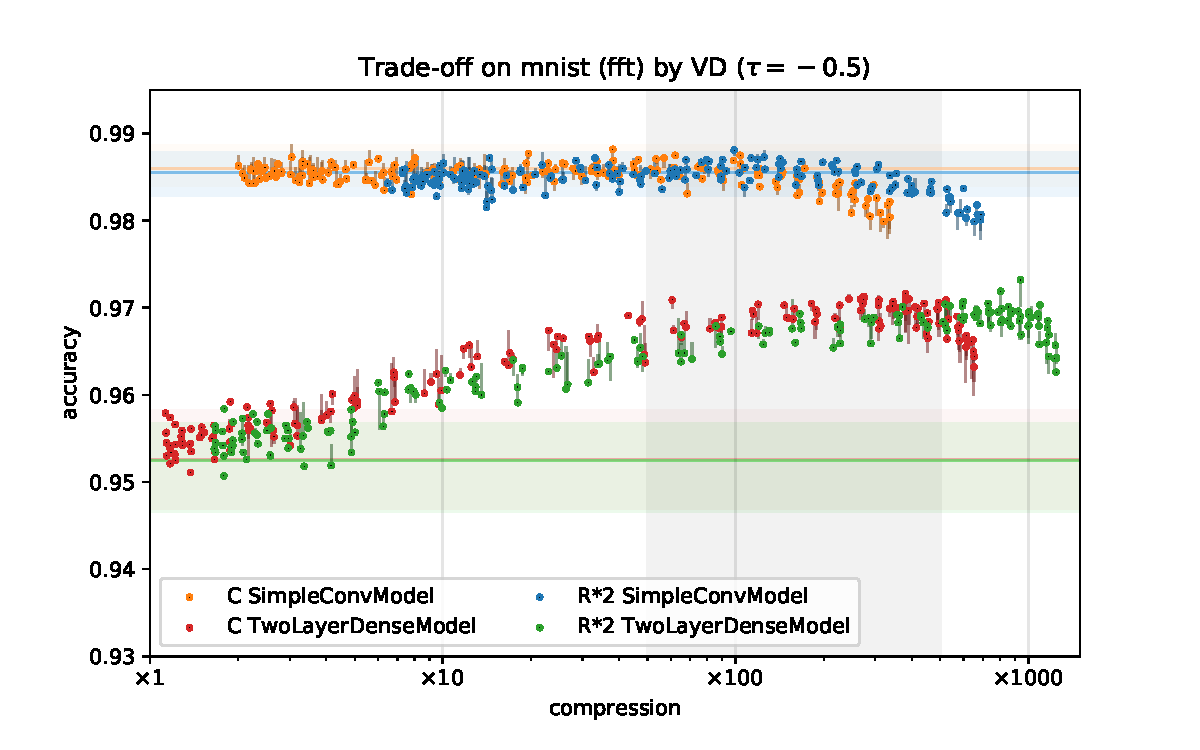
\includegraphics[width=\columnwidth]{figure__mnist-like__trade-off/appendix__cmp__VD__mnist__fft__-0.5.pdf}
  \end{subfigure} \\%
  % \hfill
  \begin{subfigure}[b]{1.\columnwidth}  % imcl2019-style swears at this
    \centering
    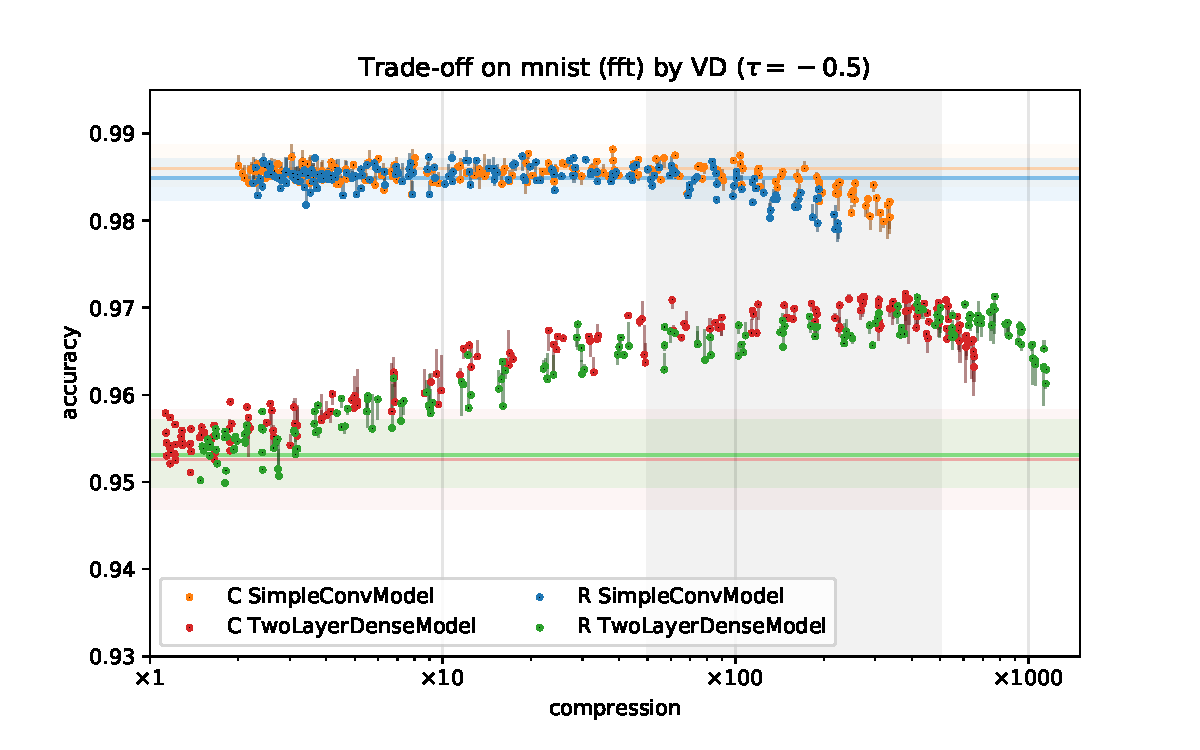
\includegraphics[width=\columnwidth]{figure__mnist-like__trade-off/appendix__VD__mnist__fft__-0.5.pdf}
  \end{subfigure}
  \caption{%
    The compression-accuracy curve (VD, \texttt{fft}, MNIST):
    $2 \real / \cplx$ (\textit{top}) and $\real / \cplx$ (\textit{bottom}).
  }
  \label{fig:mnist-like__trade-off__fft}
\end{figure}

\begin{figure}[!t]
  \centering
  \begin{subfigure}[b]{1.\columnwidth}  % imcl2019-style swears at this
    \centering
    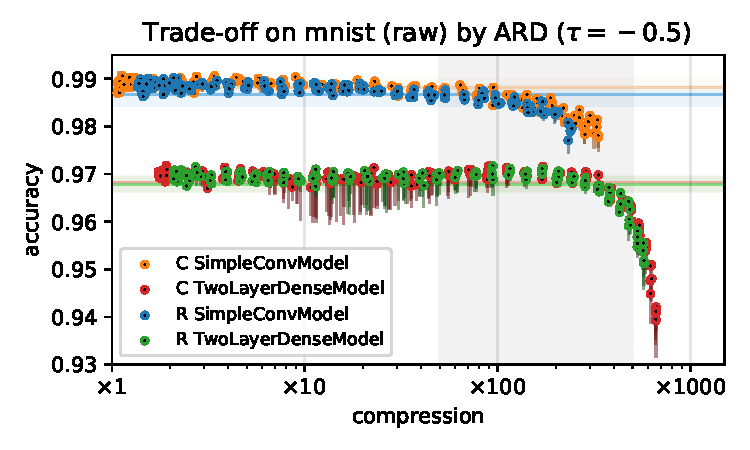
\includegraphics[width=\columnwidth]{figure__mnist-like__trade-off/appendix__ARD__mnist__raw__-0.5.pdf}
  \end{subfigure} \\%
  % \hfill
  \begin{subfigure}[b]{1.\columnwidth}  % imcl2019-style swears at this
    \centering
    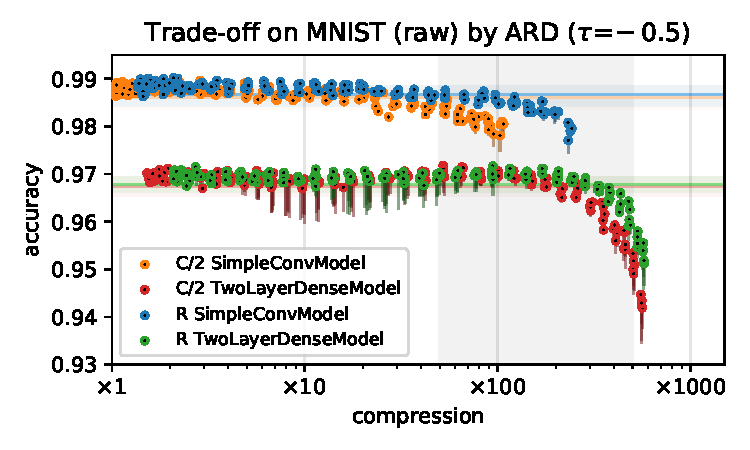
\includegraphics[width=\columnwidth]{figure__mnist-like__trade-off/appendix__cmp__ARD__mnist__raw__-0.5.pdf}
  \end{subfigure}
  \caption{%
    The compression-accuracy curve (ARD, \texttt{raw}, MNIST):
    $\real / \cplx$ (\textit{top}) and $\real / \tfrac12 \cplx$ (\textit{bottom}).
  }
  \label{fig:mnist-like__trade-off__raw}
\end{figure}

% observations
Figures~\ref{fig:mnist-like__trade-off__fft} and~\ref{fig:mnist-like__trade-off__raw}
depict the resulting compression-accuracy trade-off on MNIST for the simple models
described above (other datasets are in appendix~\ref{sec:mnist_like_experiments}).
%
The points represent the trade-off of the compressed networks after fine-tuning, while their
tails illustrate the impact of this stage on the accuracy. Transparent horizontal bands on
each plot represent min-max performance spread of an uncompressed network on the test split.

The overarching pattern in all experiments on MNIST-like datasets is that both ARD and VD
compress similarly and ARD offers marginal advantage in terms of performance after fine-tuning.
Fourier features perform marginally worse than raw image data for each model across all
compression rates, and their trade-off for the dense network has a hat-like shape, contrasting
the raw image features, for which the accuracy stays at one level for moderate rates,
and then abruptly decays in high compression regime.

The impact of ``fine-tune'' is mixed, and depends on the dataset and features, although it
frequently improves accuracy in high compression $\times50+$ (high $C$ in \eqref{eq:elbo_with_coef})
for raw image input. On EMNIST Letters and MNIST datasets in the small compression regime the
dense network exhibits a trough in accuracy before fine-tuning stage.

% conclusions
These experiments demonstrate that $\cplx$ Variational Dropout can offer adequate compression
without much loss in performance for $\cplx$-valued networks. Although ARD performs on par
with VD, unlike VD, it uses a proper prior and has a tractable analytic expression for the
KL-divergence \eqref{eq:emp-bayes-kl-div} in both $\real$ and $\cplx$ cases.
% fft: $2\real$ convolutional model trade-off overall better than $\real$, dense -- on par.
% raw: $\cplx$ models trade-off overall better than $\tfrac12\cplx$.
Wider $\real$ and $\cplx$ networks appear to have more favourable trade-off between
compression and accuracy.
% fft: any-$\real$ dense model compresses better than $\cplx$
However, it seems that due to more intrinsic degrees of freedom, $\real$-valued models
perform and compress better than $\cplx$, even when the former uses the same number of
features as the latter.
% $\cplx$-valued networks do not have as much spare capacity as $2 \real$ due to
%  constraints imposed by multiplication in $\cplx$ numbers

% subsection mnist_like_datasets (end)


\subsection{CIFAR10} % (fold)
\label{sub:cifar10}

We conduct an experiment on the CIFAR10 classification dataset \citep{krizhevsky_learning_2009}
comprising $32\times 32$ color images of $10$ classes to study the performance-compression
trade-off of a moderately large deep network.
% same experimental setup as in MNIST, describe the VGG16 model and its cplx-valued modification
The experiment is set up similarly to MNIST-like experiment, except that we train $\real$
VGG16 network \citep{simonyan_very_2015} and its $\cplx$ variant, in which we have replaced
$\real$-valued layers with their $\cplx$-valued counterparts. $\real$ and $\cplx$ VGG16 have
the same feature sizes in intermediate layers.

% differences with mnist
Unlike experiment in sec.~\ref{sub:mnist_like_datasets}, we consider the raw features only,
use full training split, and allocate $20$, $40$, and $20$ epochs to each stage. During training
the mini-batch of $128$ samples is randomly augmented by randomly flipping horizontally and
cropping. Random cropping is done by zero-padding each side by four pixels and extracting a
random $32\times 32$ patch from the $40\times 40$ intermediate image.
%
We vary $C$ in \eqref{eq:elbo_with_coef} over $
  \{\tfrac32 2^{-\tfrac{k}2} \colon k=7, \cdots, 15\}
$, compare VD and ARD methods, and measure accuracy on CIFAR10 test split.

% compare compressed cplx-vgg against real-vgg
\begin{figure}[!t]
  \centering
  \begin{subfigure}[b]{1.\columnwidth}  % imcl2019-style swears at this
    % 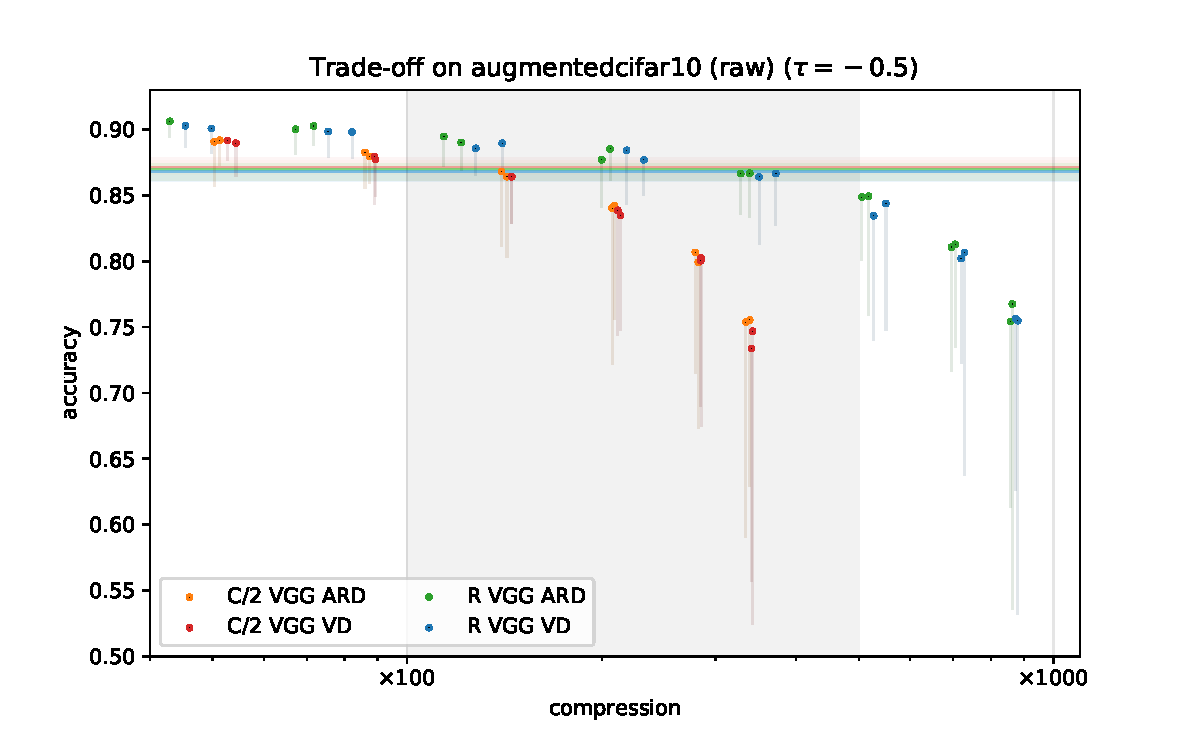
\includegraphics[width=\columnwidth]{figure__cifar__trade-off/legacy__augmentedcifar10__raw__-0.5.pdf}
    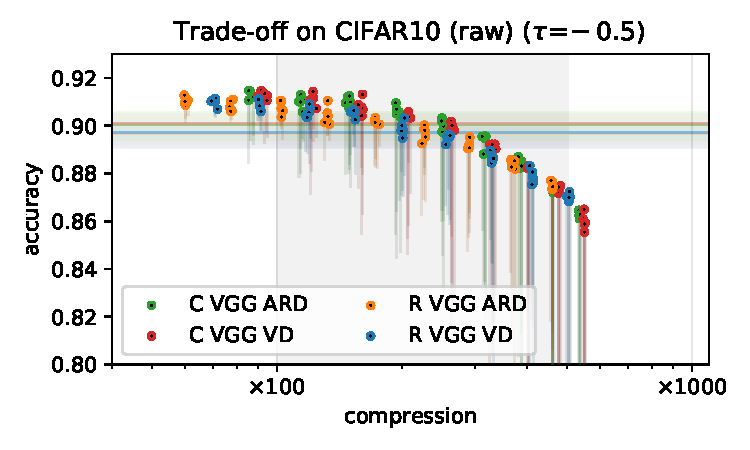
\includegraphics[width=\columnwidth]{figure__cifar__trade-off/appendix__augmentedcifar10__raw__-0.5.pdf}
  \end{subfigure}
  \caption{%
    The compression-accuracy frontier for VGG16 ($\real$ and $\cplx$) on CIFAR10.
  }
  \label{fig:figure__cifar10__trade-off}
\end{figure}

% draw some conclusions
Figure~\ref{fig:figure__cifar10__trade-off} shows that, although ARD method offers slightly
less compression, it makes up for it by marginally better accuracy post fine-tune. VGG16 and
$\cplx$-VGG16 exhibit similar declining compression-accuracy trade-off, but due to higher
capacity $\cplx$-valued network yields higher accuracy \citep{monning_evaluation_2018}. Unlike
MNIST, fine-tuning stage significantly improves the test performance, which, we speculate, might
be due to dataset augmentation and deeper model.
% reword this sentence

% subsection cifar10_100 (end)


\subsection{MusicNet} % (fold)
\label{sub:musicnet}

% describe musicnet as in Trabelsi et al. (2017) also get some hints from thickstun_learning_2017
We use MusicNet \citep{thickstun_learning_2017}, an audio dataset of $330$ annotated
musical compositions, to investigate compressibility of the $1d$ VGG-like $\cplx$-convent
proposed by \citet{trabelsi_deep_2018}. Similarly to the study, we downsample the audio
from 44.1kHz to 11kHz, retain only $84$ out of $128$ labels, and hold-out the same validation
and test compositions, on which we score the models with the pooled average precision.
Each epoch lasts for $1000$ random mini-batches of the remaining $321$ pieces. The input
features are $\cplx$-valued Fourier transformed windows of $4096$ samples from each waveform.
The label vectors are taken from annotations at the middle of the window.

Experiments with the uncompressed model aimed at replicating the result of \citet{trabelsi_deep_2018}
have shown that early stopping almost always terminates much sooner, than $200$ epochs used
in their study: within the first $10-20$ epochs with the validation performance peaking at
$10-15$ epochs and steadily declining afterwards.
%
Thus we opt to use shorter stages: $12$, $32$ and $50$ epochs (sec.~\ref{sub:staging}), with
early stopping activated only during the ``fine-tune'' stage. To keep the learning rate schedule
consistent, we scale the learning rate of $10^{-3}$ after $5$, $10$, and $20$-th epoch by
$\tfrac1{10}$, $\tfrac1{20}$ and $\tfrac1{100}$, respectively.

We deviate from the set-up used by \citet{trabelsi_deep_2018} by clipping $\ell_2$ norm of the
gradients to $0.05$ and shifting the low frequencies of the input to the centre to maintain
spatial locality for convolutions.

We test complex ARD (sec.~\ref{ssub:ard_prior}) and VD (sec.~\ref{ssub:vd_prior}) methods
and vary $
  C \in \{\tfrac14, \tfrac12, \tfrac34, 1\} \cdot 10^{-k}
$ for $k=1, 2, 3$, while keeping $\tau$ at $-\tfrac12$. The performance is measured after
``dense'' stage, before the beginning and upon termination of fine-tuning.
%
Additionally, we test the model of \citet{trabelsi_deep_2018}, in which we purposefully
halve the receptive field of the first convolution from $6$ to $3$ (denoted by suffix $k_3$).
The motivation is to test if the handicap introduced by the forced compression of the most
upstream layer can be alleviated by non-uniform compression, induced by variational dropout.
We test only complex VD in this sub-experiment, since prior results have not demonstrated
significant superiority of one method over another.  % it should've been ARD

\begin{figure}[!t]
  \centering
  \begin{subfigure}[b]{1.\columnwidth}  % imcl2019-style swears at this
    \centering
    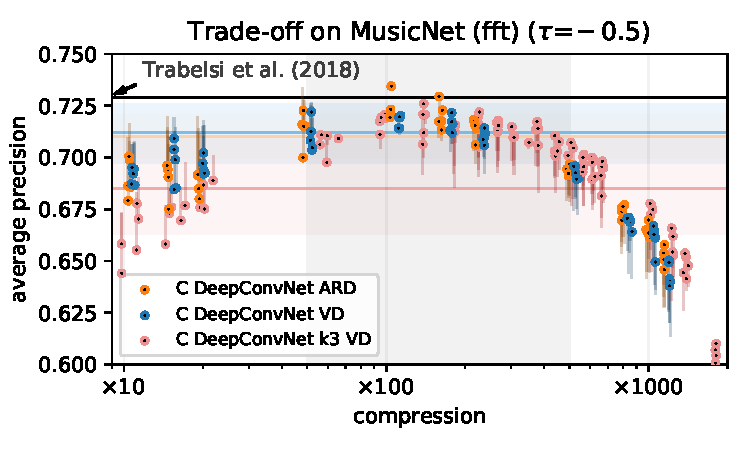
\includegraphics[width=\columnwidth]{figure__musicnet__trade-off/paper__musicnetram__fft__-0.5.pdf}
  \end{subfigure}
  \caption{%
    Performance-compression curve for \textbf{\color{blue} VD}, \textbf{\color{orange} ARD},
    and the ${\color{gray} k_3}$ version compressed with VD.
  }
  \label{fig:musicnet__trade-off}
\end{figure}

Figure~\ref{fig:musicnet__trade-off} shows the resulting performance-compression frontier.
ARD slightly outperforms VD in terms of performance, but both deliver similar compression
rates. The trade-off demonstrates that with the proposed $\cplx$-valued variational dropout
methods (sec.~\ref{sec:c_variational_dropout}) and post-sparsification fine-tuning it is
possible to achieve average precision level comparable to the result of \citet{trabelsi_deep_2018}
with a model compressed $50\times$-$200\times$. Furthermore, the $k_3$ model, compressed
$110 \times$ with $\cplx$ VD, outperforms its uncompressed baseline, but yields lower
performance than the full model.

\begin{figure}[!t]
  \centering
  \begin{subfigure}[b]{1.\columnwidth}  % imcl2019-style swears at this
    \centering
    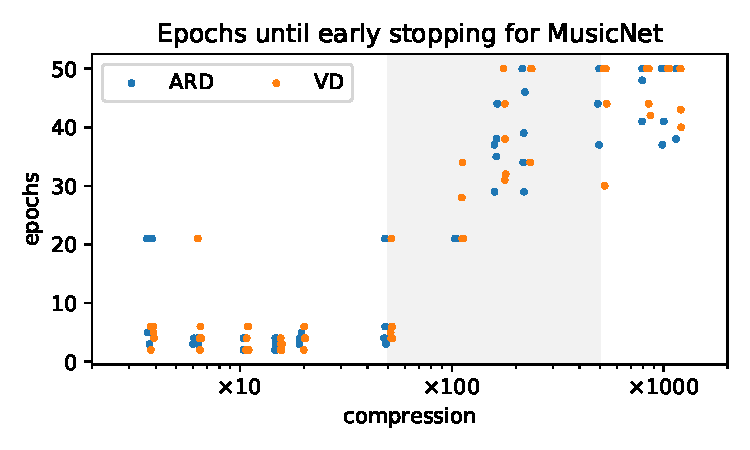
\includegraphics[width=\columnwidth]{figure__fine-tune_fx__early__compression.pdf}
  \end{subfigure}
  \caption{%
    Early stopping epoch at fine-tuning stage.
  }
  \label{fig:musicnet__early_stopping}
\end{figure}

% why is there such a dramamtic difference in impact of ``fine-tune''?
We provide the following interpretation of the apparent difference in performance impact
of the ``fine-tune'' stage between less than $50\times$ and higher than $100\times$ compression
regimes in figure~\ref{fig:musicnet__trade-off}, also observed in sec.~\ref{sub:mnist_like_datasets}.
%
% * early stopping kick in at around 10-20 epoch
% * performance peaks at 10-15 epoch and then gradually declines
The value of $C$ in \eqref{eq:elbo_with_coef} is a good proxy for the ranking of the final
compression rate since it directly affects the feedback from sparsifying prior. So, with
low $C$ models get less compressed during $50$ epoch allotted for ``sparsify'' stage, which
appears to be insufficient to move model away from the parameters after the dense stage.
It is reasonable therefore to expect that for undercompressed models the fine-tuning stage
acts essentially as a continuation of the pre-training stage. Since we have observed that
longer training invariably deteriorates the validation performance, the ``fine-tune'' stage
leads to overfitting. Figure~\ref{fig:musicnet__early_stopping}, which shows that the models,
which have been sparsified with $C$ less than $\tfrac1{400}$ and have $50\times$ compression,
need considerably less training epochs before early stopping terminates the process.

% testing the fx of the threshold
\begin{figure}[!t]
  \centering
  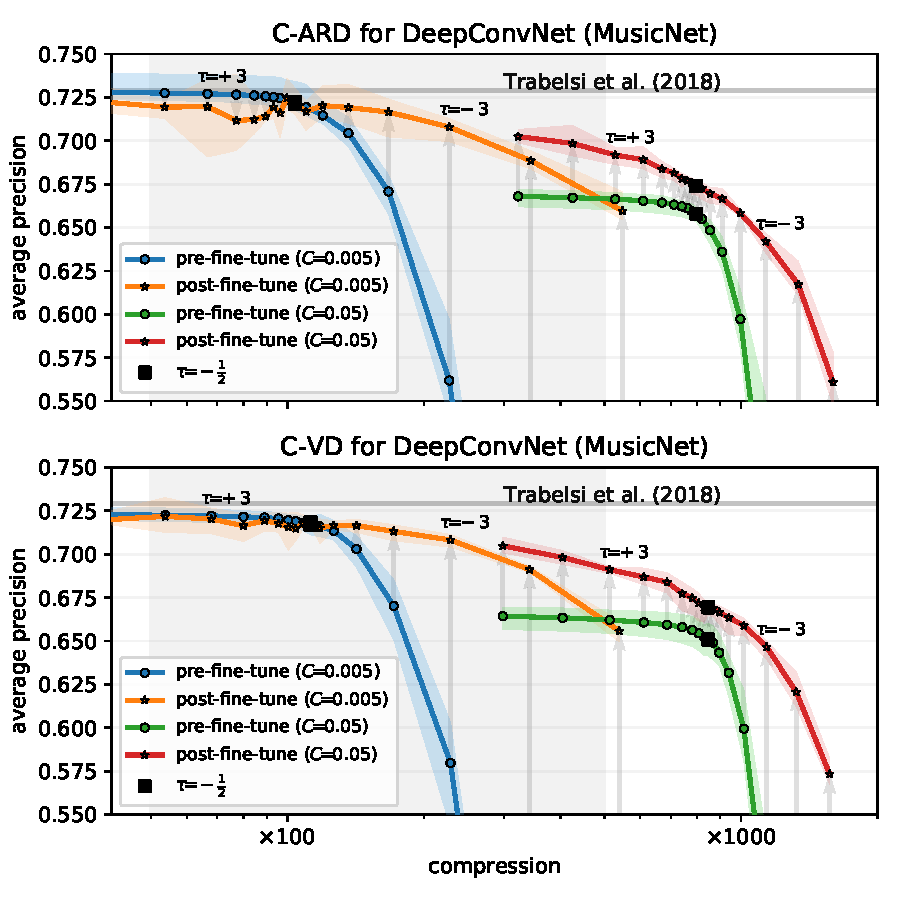
\includegraphics[width=1\columnwidth]{figure__musicnet__threshold__C__DeepConvNet.pdf}
  \caption{%
    Effects of finetunig on performance-compression curves parameterized by $
      \tau\in \{\tfrac{k}2\colon k=-8..+8 \}
    $ for $
      C\in \{\tfrac1{20}, \frac1{200}\}
    $ in \eqref{eq:elbo_with_coef} during sparsification (sec.~\ref{sub:staging}).
  }
  \label{fig:hist__and__threshold__tradeoff}
\end{figure}

% effects of extra training epochs and the impact of tau
We take the models from experiments with $C \in \{\tfrac1{20}, \frac1{200}\}$ and plot
the compression and performance metrics before fine-tuning for various threshold levels
on figure~\ref{fig:hist__and__threshold__tradeoff} (top). From \eqref{eq:elbo_with_coef} and
the relative positions of the compression curves it can be concluded that $C$ has much
more substantial impact on the sparsity and performance, than the choice of $\tau$.
Furthermore, for $\tau > 0$ the performance quickly saturates while compression creeps
downwards.
%
The bottom plot in figure~\ref{fig:hist__and__threshold__tradeoff} shows the effect of
the ``fine-tune'' stage: for $\tau \leq -1$ it improves the test performance, while leaving
it mostly unaffected for positive $\tau$. We attrbute this behaviour to regularization
effect of high compression rate, which limits the capacity for overfitting by significantly
reducing the excess degrees of freedom.
% coarser grid than in top plot in order not to wait for 20 compute days, but 9.5 on
% 4 x Geforce 1080Ti, 256 Gb, core-i7 machine, running 4*2 experiments in parallel

% takeaway: fine tune seems to improve performance for highly compressed models, but
% within a limit. Worth a try for moderately compressed models, but willl must likely
% overfit for undercompressed models. Varying $C$ in \eqref{eq:elbo_with_coef} affects
% sparsity more strongly, than varying $\tau$. But this is only observational.

% subsection musicnet (end)

% section experiments (end)


\section{Conclusion} % (fold)
\label{sec:conclusion}

In this study we have extended Variational Dropout methods of \citet{kingma_variational_2015},
\citet{molchanov_variational_2017} and \citet{kharitonov_variational_2018} to $\cplx$-valued
Bayesian networks. To validate the proposed technique we have conducted a large numerical
study of complex-valued networks with simple architectures in image recognition tasks to
assess the feasible performance-compression trade-off. At the cost of marginally lower performance,
we have achieved $50-100\times$ compression of the state-of-the-art deep $\cplx$-valued network
of \citet{trabelsi_deep_2018} on the MusicNet.

The results of this study have direct implications for real-time signal processing with
embedded deep learning applications both in terms of lower storage requirements and higher
throughput stemming from fewer floating-point multiplications, despite higher arithmetic
complexity of $\cplx$-valued networks.

% section conclusion (end)

% \clearpage

\bibliographystyle{abbrvnat}
\bibliography{references}
% \nocite{*}

% \clearpage

\appendix
\onecolumn

\section{Gradient of the KL-divergence in $\real$ case} % (fold)
\label{sec:real-chisq-grad}  % gradient_of_the_kl_divergence_in_R_case

In this section we derive the exact gradient of \eqref{eq:improper-kl-div-real}. Even
though, ultimately, the divergence involves a hypergeometric function, and its gradient
requires evaluating the Gauss error function, the analysis provides independent verification
of the approximation, proposed by \citet{molchanov_variational_2017}. The logic of the
derivation follows \citet{lapidoth_capacity_2003}.
% \citet{pav_moments_2015} correctly notice that \cite[p. 2466]{lapidoth_capacity_2003} has a missing $\log{2}$ term.

For $(z_i)_{i=1}^m \sim \mathcal{N}(0, 1)$ iid and $
  (\mu_i)_{i=1}^m \in \mathbb{R}
$, the random variable $W = \sum_i (\mu_i + z_i)^2$ is noncentral $\chi^2$ with shape $m$
and noncentrality parameter $\lambda = \sum_i \mu_i^2$, i.e. $W\sim \chi^2_m(\lambda)$.
Its density is
\begin{equation}  \label{eq:nonchisq-density}
  f_W(x)
    % = e^{- \tfrac\lambda2} \sum_{n \geq 0} \tfrac{\bigl(\tfrac\lambda2\bigr)^n}{n!}
    %   \tfrac{
    %     x^{n + \tfrac{m}2 - 1} e^{-\tfrac{x}2}
    %   }{
    %     2^{n + \tfrac{m}2} \Gamma(n + \tfrac{m}2)
    %   }
    % = e^{- \tfrac\lambda2} \sum_{n \geq 0} \tfrac{\bigl(\tfrac\lambda2\bigr)^n}{n!}
    %     \tfrac{
    %         \bigl(\tfrac{x}2\bigr)^{n + \tfrac{m}2 - 1} e^{-\tfrac{x}2}
    %     }{
    %         2 \Gamma(n + \tfrac{m}2)
    %     }
    = \frac12 e^{- \tfrac{x + \lambda}2} \bigl(\tfrac{x}2\bigr)^{\tfrac{m}2 - 1}
      \sum_{n \geq 0} \frac{
        \bigl(\tfrac{x \lambda}4\bigr)^n
      }{
        n! \Gamma(n + \tfrac{m}2)
      }
    % = \frac12 e^{- \tfrac{x + \lambda}2}
    % \bigl(\tfrac{x}\lambda\bigr)^{\tfrac{m}4 - \tfrac12}
    % \bigl(\tfrac{x \lambda}4\bigr)^{\tfrac{m}4 - \tfrac12}
    % \sum_{n \geq 0} \tfrac{
    %         \bigl(\tfrac{x \lambda}4\bigr)^n
    %     }{
    %         n! \Gamma(n + \tfrac{m}2)
    %     }
    % = \frac12 e^{- \tfrac{x + \lambda}2}
    % \bigl(\tfrac{x}\lambda\bigr)^{\tfrac{m}4 - \tfrac12}
    % \bigl(\tfrac{\sqrt{x \lambda}}2\bigr)^{\tfrac{m}2 - 1}
    % \sum_{n \geq 0} \tfrac{
    %         \bigl(\tfrac{x \lambda}4\bigr)^n
    %     }{
    %         n! \Gamma(n + \tfrac{m}2)
    %     }
    % = \frac12 e^{- \tfrac{x + \lambda}2}
    % \bigl(\tfrac{x}\lambda\bigr)^{\tfrac{m - 2}4}
    % I_{\bigl(\tfrac{m}2 - 1\bigr)}(\sqrt{x \lambda})
    \,.
\end{equation}
% where $I_k$ is the modified Bessel function of the first kind
% $$
% I_k(s)
%   = \Bigl(\frac{s}2\Bigr)^k
%       \sum_{n \geq 0} \tfrac{
%           \bigl( \tfrac{s}2 \bigr)^{2n}
%       }{n! \Gamma(n + k + 1)}
%   \,. $$
By integrating the power series \eqref{eq:nonchisq-density} with substitution $x \to 2u$,
the expectation $
  \mathbb{E}_{W\sim \chi^2_m(\lambda)} \log W
$, needed in \eqref{eq:improper-kl-div-real}, equals
\begin{multline}  \label{eq:exp-log-chisq-proof}
    % &= \int_0^\infty f_W(x) \log x dx
    % \notag \\
    % &\frac12 e^{- \tfrac\lambda2}
    % \int_0^\infty \sum_{n \geq 0} \biggl(
    %     \frac{
    %       e^{- \tfrac{x}2} \bigl(\tfrac\lambda2\bigr)^n
    %     }{
    %       n! \Gamma(n + \tfrac{m}2)
    %     }
    %     \bigl(\tfrac{x}2\bigr)^{n + \tfrac{m}2 - 1}
    % \biggr) \log{(x)} dx
    % = [\text{ absolute summability and Fubini, or any other conv. thm for integrals of nonnegative integrals}]
    % = e^{- \tfrac\lambda2} \sum_{n \geq 0}
    %     \tfrac{\bigl(\tfrac\lambda2\bigr)^n}{n!}
    %     \tfrac1{\Gamma(n + \tfrac{m}2)}
    % \int_0^\infty
    %     e^{- \tfrac{x}2} \bigl(\tfrac{x}2\bigr)^{n + \tfrac{m}2 - 1}
    %     (\log2 + \log \tfrac{x}2) \tfrac{dx}2
    % = [u = \tfrac{x}2]
    % \notag \\
    e^{- \tfrac\lambda2} \sum_{n \geq 0}
        \frac{\bigl(\tfrac\lambda2\bigr)^n}{
          n! \Gamma(n + \tfrac{m}2)
        }
    \int_0^\infty
        e^{- u} u^{n + \tfrac{m}2 - 1}
        \log{(2 u)} du
    % = [\text{definitions:} \Gamma, \psi]
    % = e^{- \tfrac\lambda2} \sum_{n \geq 0}
    %     \tfrac{\bigl(\tfrac\lambda2\bigr)^n}{n!}
    % (\psi(n + \tfrac{m}2) + \log2)
    % \notag
    \\
    = \log{2}
    + e^{- \tfrac\lambda2} \sum_{n \geq 0}
        \frac{\bigl(\tfrac\lambda2\bigr)^n}{n!}
        \psi(n + \tfrac{m}2)
    \,,
\end{multline}
where $\psi(x)$ is the digamma function, i.e.
\begin{equation}  \label{eq:digamma}
  \psi(x)
    % = \frac{d}{dx} \log \Gamma(x)
    = \frac1{\Gamma(x)}
      \int_0^\infty
        u^{x-1} e^{-u} \log{u}
      \, du
    \,,
\end{equation}
which satisfies $
  \psi(z+1) = \psi(z) + \tfrac1z
$, $
  \psi(x)\leq \log x - \tfrac1{2x}
$, and $
  \psi(\tfrac12) = -\gamma - 2\log 2
$ ($\gamma$ is Euler's constant). If we put
\begin{equation}  \label{eq:g-m-series}
  g_m(x)
    % alpha: e^{-x} \sum_{n=0}^{\infty} \frac{x^n}{n!} \psi(n + m / 2)
    % = e^{-x} \sum_{n \geq 0} \frac{x^n}{n! \Gamma(n + \tfrac{m}2)}
    %     \int_0^\infty e^{-t} t^{n + \tfrac{m}2-1} \log{t} dt
    = e^{-x} \sum_{n \geq 0} \frac{x^n}{n!} \psi(n + \tfrac{m}2)
    \,,
\end{equation}
then the desired expectation in \eqref{eq:improper-kl-div-real} equals $
  \log{2} + g_1(\tfrac1{2\alpha})
$.
%
% We can differentiate the series in $g_m(x)$, since the sum converges on $\mathbb{R}$.
% Indeed, it is a power series featuring nonnegative coefficients, which is dominated by $
%   \sum_{n \geq 1} \tfrac{x^n}{n!} \log{(n+\tfrac{m}2)}
% $. By the ratio test, the dominating
% series has infinite radius:
% $$
% \lim_{n\to\infty}
%   \biggl\lvert
%     \frac{
%       n! x^{n+1} \log{(n + 1 + \tfrac{m}2)}
%     }{
%       x^n \log{(n + \tfrac{m}2)} (n+1)!
%     }
%   \biggr\rvert
%   = \lim_{n\to\infty}
%     \lvert x \rvert 
%     \biggl\lvert
%       \frac{
%         \log{(n + 1 + \tfrac{m}2)}
%       }{
%         \log{(n + \tfrac{m}2)} (n+1)
%       }
%     \biggr\rvert
%   % = \lim_{n\to\infty}
%   %   \lvert x \rvert 
%   %   \biggl\lvert
%   %     \frac{
%   %       n + \tfrac{m}2
%   %     }{
%   %       (n + 1 + \tfrac{m}2)((n+1) + (n + \tfrac{m}2) \log{(n + \tfrac{m}2)})
%   %     }
%   %   \biggr\rvert
%   = 0 < 1
%   \,, $$
% since
% $$
% \frac{\log{(x + a + 1)}}{x \log{(x + a)}}
%   \sim \frac{\log{(x+1)}}{(x-a) \log{x}}
%   \sim \frac{\log{(x+1)}}{x \log{x}}
%   \sim \frac{\tfrac1{(x+1)}}{1 + \log{x}}
%   \to 0
%   \,. $$
% A theorem from calculus states, that the formal series derivative (integral)
% coincides with the derivative (integral) of the function, corresponding to
% the power series (everywhere on the convergence region). And the convergence
% regions of derivative (integral) coincide with the region of the original
% power series.
%
Formally differentiating the convergent power series within $g_m$ yields
\begin{equation}  \label{eq:g-m-deriv}
  \frac{d}{d x} g_m(x)
    % = e^{-x} \sum_{n\geq 1} \frac{x^{n-1}}{(n-1)!} \psi(n + \tfrac{m}2) - g_m(x)
    % = e^{-x} \sum_{n\geq 0} \frac{x^n}{n!} \psi(n + \tfrac{m}2 + 1) - g_m(x)
    % = e^{-x} \sum_{n\geq 0} \frac{x^n}{n!} (
    %     \psi(n + \tfrac{m}2 + 1) - \psi(n + \tfrac{m}2)
    % )
    % = e^{-x} \sum_{n\geq 0} \frac{x^n}{n!} \tfrac1{n + \tfrac{m}2}
    % = e^{-x} \sum_{n\geq 0} \frac{x^n}{n!} (n + \tfrac{m}2)^{-1}
    = x^{-\tfrac{m}2} e^{-x} \sum_{n\geq 0}
        \frac{x^{n + \tfrac{m}2}}{n!} (n + \tfrac{m}2)^{-1}
    \,.
\end{equation}
From $
    e^t  = \sum_{n\geq 0} \tfrac{t^n}{n!}
$ on $\mathbb{R}$ and $
  \tfrac{x^\alpha}{\alpha}
    = \int_0^x t^{\alpha-1} dt
$ for $\alpha\neq 0$ we get
% by the monotone convergence theorem on ([0, x], \mathcal{B}([0, x]), dx)
\begin{align}  \label{eq:g-m-deriv-int-2}
  \eqref{eq:g-m-deriv}
    % = x^{-\tfrac{m}2} e^{-x} \sum_{n\geq 0}
    %     \frac{x^{n + \tfrac{m}2}}{n!} (n + \tfrac{m}2)^{-1}
    &= x^{-\tfrac{m}2} e^{-x} \sum_{n\geq 0}
        \frac1{n!} \int_0^x t^{n + \tfrac{m}2 - 1} dt
    % = x^{-\tfrac{m}2} e^{-x}
    %     \int_0^x t^{\tfrac{m}2 - 1} \sum_{n\geq 0} \frac{t^n}{n!} dt
    \notag \\
    &= x^{-\tfrac{m}2} e^{-x}
        \int_0^x t^{\tfrac{m}2 - 1} e^t dt
    \,.
\end{align}
Substitution $u^2 = t$ on $[0, \infty]$ with $2u du = dt$ yields
\begin{equation}  \label{eq:g-m-deriv-int-3}
  \frac{d}{d x} g_m(x)
    % = x^{-\tfrac{m}2} e^{-x}
    %     \int_0^x t^{\tfrac{m}2 - 1} e^t dt
    = 2 x^{-\tfrac{m}2} e^{-x}
        \int_0^{\sqrt{x}} u^{m - 1} e^{u^2} du
    \,.
\end{equation}
In particular, the derivative of \eqref{eq:g-m-series} for $m=1$ is
\begin{equation}  \label{eq:g-m-deriv-one}
  \frac{d}{d x} g_1(x)
    = 2 \frac{F(\sqrt{x})}{\sqrt{x}}
    \,,
\end{equation}
using Dawson's integral $
  F
  % \colon \mathbb{R} \to \mathbb{R}
  \colon x \mapsto e^{-x^2} \int_0^x e^{u^2} du
$.
%
Hence, the derivative of the expectation in \eqref{eq:improper-kl-div-real} with respect
to $\alpha$ is
$$
\frac{d}{d \alpha} g_1(\tfrac1{2\alpha})
  = -\frac1{2 \alpha^2} g_1'(\tfrac1{2\alpha})
  % = -\frac1{2 \alpha^2} 2 \tfrac{F(\sqrt{\tfrac1{2\alpha}})}{\sqrt{\tfrac1{2\alpha}}}
  % = -\frac1{2 \alpha^2} 2 \tfrac{F(\tfrac1{\sqrt{2\alpha}})}{\tfrac1{\sqrt{2\alpha}}}
  = -\frac1{\alpha} \sqrt{\frac2{\alpha}} F(\tfrac1{\sqrt{2\alpha}})
  \,. $$
Finally, since $\alpha$ is nonnegative, it is typically parameterized via its logarithm.
The gradient of \eqref{eq:improper-kl-div-real} w.r.t $\log \alpha$ is
\begin{equation}  \label{eq:real-kl-div-deriv-log}
  \frac{d \eqref{eq:improper-kl-div-real}}{d\log \alpha}
  % \frac{d}{d\log \alpha}
  %   \frac12 \mathbb{E}_{z \sim \mathcal{N}(0,1)}
  %     \log \lvert z + \tfrac1{\sqrt{\alpha}} \rvert^2
    % = \frac12 \frac{d\alpha}{d\log \alpha}
    %   \frac{d}{d\alpha} \bigl(\mathbb{E}\cdots \bigr)
    % = - \frac\alpha2 \tfrac1{\alpha}
    %   \sqrt{\tfrac2{\alpha}} F(\tfrac1{\sqrt{2\alpha}})
    = - \frac1{\sqrt{2\alpha}} F\bigl(\tfrac1{\sqrt{2\alpha}}\bigr)
    \,.
\end{equation}

We compute the Monte-Carlo estimator of \eqref{eq:improper-kl-div-real} on a sample of $10^7$
draws over an equally spaced grid of $\log \alpha$ in $[-12, +12]$ of size $4096$. The
coefficients of the approximation, proposed by \citet{molchanov_variational_2017}, are
within $1\%$ relative tolerance of the reported therein. An equivalent expression of the
approximation is given in \eqref{eq:improper-kl-div-real-approx}.
% see eq.~(14): flit overall sign, use $C = -k_1$, $1-\sigma(x) = \sigma(-x)$
\begin{equation}  \label{eq:improper-kl-div-real-approx}
  \eqref{eq:improper-kl-div-real}
% - KL(\mathcal{N}(w \mid \mu, \alpha \mu^2) \|
%     \tfrac1{\lvert w \rvert})
%   \approx
%     k_1 \sigma(k_2 + k_3 \log \alpha)
%     + C \big\vert_{C = -k1}
%     - \tfrac12 \log (1 + e^{-\log \alpha})
  % = \tfrac12 \log \alpha
  %   - \mathbb{E}_{\xi \sim \mathcal{N}(1, \alpha)}
  %   \log{\lvert \xi \rvert} + C
  \approx
    \frac12 \log{\bigl(1 + e^{-\log \alpha}\bigr)}
    + k_1 \sigma\bigl(- (k_2 + k_3 \log \alpha)\bigr)
    % - k_1 \bigl(1 - \sigma(k_2 + k_3 \log \alpha)\bigr)
  \,,
\end{equation}
% in parctial implementations we suggest using softplus to numerically comptue the last
% term, since it is typically implemented in a floating-point stable fashion.
The numerically estimated derivative of the penalty term with respect to $\log \alpha$ using
forward differences seems to be following \eqref{eq:real-kl-div-deriv-log} very closely (up to
sampling error), see fig.~\ref{fig:molchanov-derivative-replica}. The derivative of
\eqref{eq:improper-kl-div-real-approx} with respect to $\log \alpha$ appears to be very close
to \eqref{eq:real-kl-div-deriv-log}. We compute a similar Monte-Carlo estimate for
$\cplx$ variational dropout KL divergence term in \eqref{eq:c-vd-kl-div} with $\beta = 2$,
fit the best approximation \eqref{eq:improper-kl-div-real-approx}, and compare the derivatives.

\begin{figure}[!t]
  \centering
  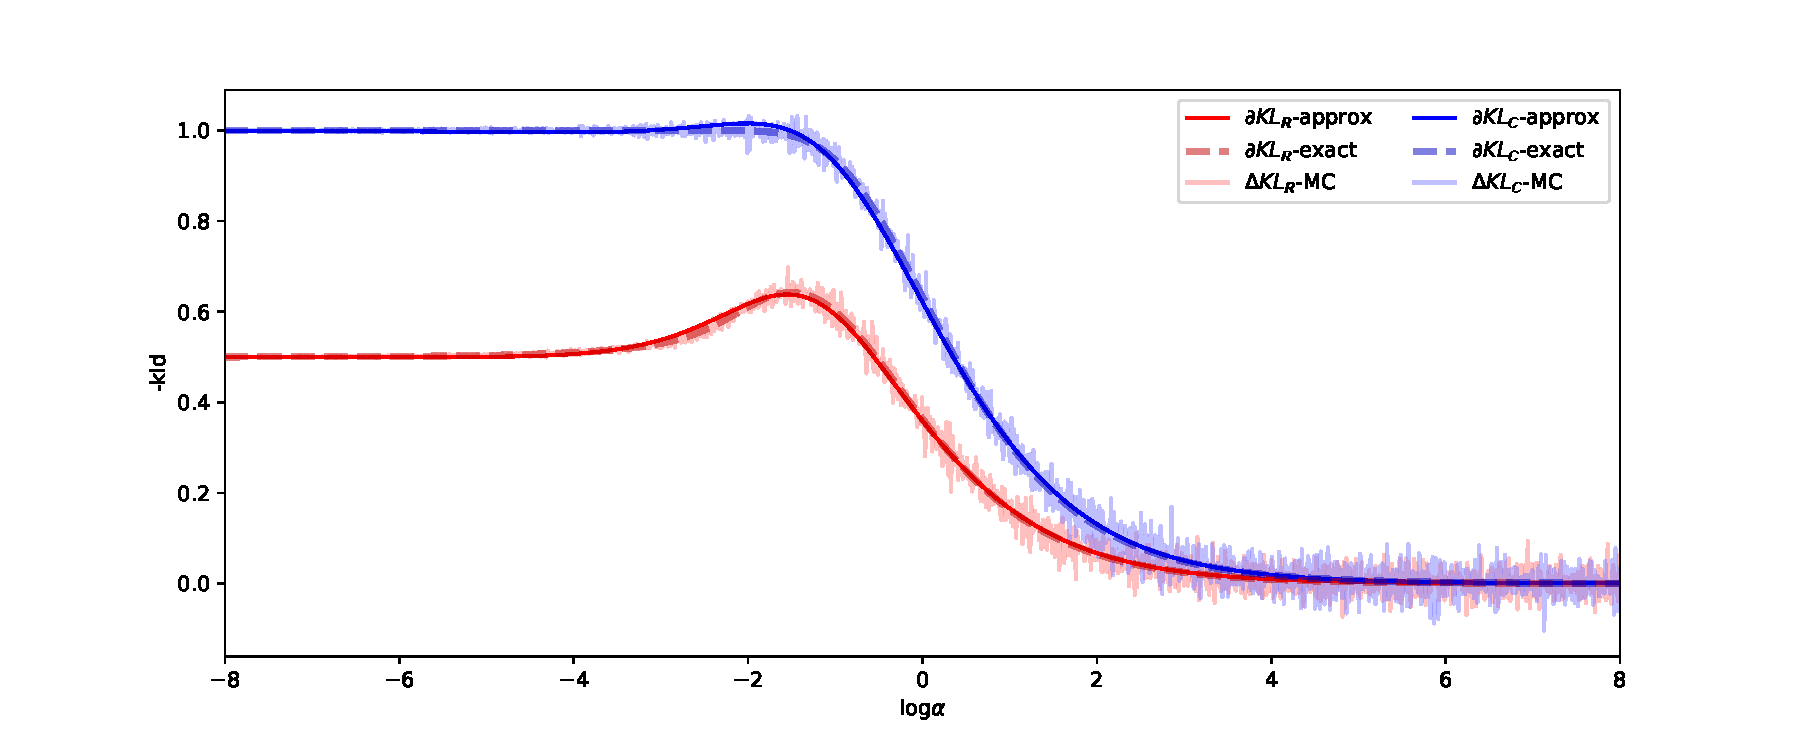
\includegraphics[width=\columnwidth]{grad_log.pdf}
  \caption{$\tfrac{d f(\alpha)}{d \log{\alpha}}$ of the approximation
  \eqref{eq:improper-kl-div-real-approx}, MC estimate of \eqref{eq:improper-kl-div-real},
  and the exact derivative using \eqref{eq:real-kl-div-deriv-log}.}
  \label{fig:molchanov-derivative-replica}
\end{figure}

% section real-chisq-grad (end)

\section{MNIST-like experiments} % (fold)
\label{sec:mnist_like_experiments}

The plots presented in this appendix support the conclusions made in the main text and
provide an overview of the experiments conducted on MNIST-like datasets.

Each figure shows the compression-accuracy trade-off of a particular method and input
features for \emph{SimpleConvModel} and \emph{TwoLayerDenseModel} models for all four
of the studied datasets (described in the main text): EMNIST-Letters on the \emph{top-left},
KMNIST -- \emph{top-right}, Fashion MNIST -- \emph{bottom-left}, and MNIST on the
\emph{bottom-right}.
%
Figures \ref{fig:appendix__mnist-like__trade-off__ARD__fft}, \ref{fig:appendix__mnist-like__trade-off__VD__fft},
\ref{fig:appendix__mnist-like__trade-off__ARD__raw}, and \ref{fig:appendix__mnist-like__trade-off__VD__raw}
present $\real$ and $\cplx$ models with \emph{the same intermediate feature sizes}.

We also report the trade-off comparison, when the argument by \citet{monning_evaluation_2018}
for higher intrinsic capacity of $\cplx$-valued networks has been taken into account.
%
We compare $\real$ networks against $\tfrac12 \cplx$ with half the number of parameters
for raw input features on figures \ref{fig:appendix__cmp__mnist-like__trade-off__ARD__raw},
and \ref{fig:appendix__cmp__mnist-like__trade-off__VD__raw}, and $2 \real$ with
double the number of parameters against $\cplx$ for Fourier input features on figures
\ref{fig:appendix__cmp__mnist-like__trade-off__ARD__fft} and
\ref{fig:appendix__cmp__mnist-like__trade-off__VD__fft}.

\begin{figure}[b]
  \centering
  \begin{subfigure}[b]{0.5\columnwidth}
    \centering
    % used in main text
    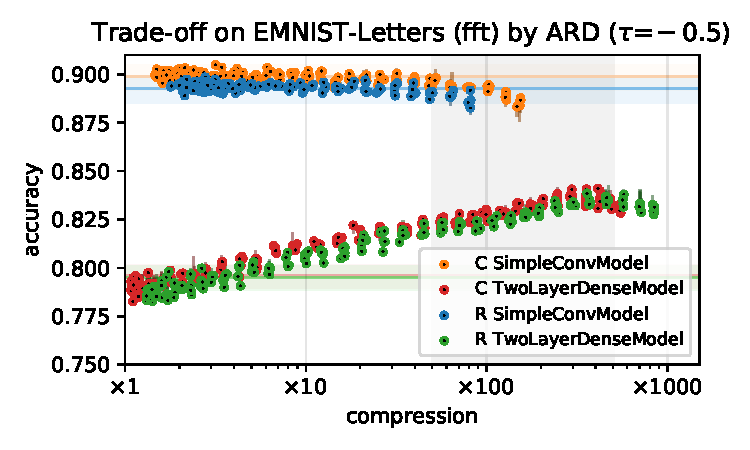
\includegraphics[width=\linewidth]{figure__mnist-like__trade-off/appendix__ARD__emnist_letters__fft__-0.5.pdf}
  \end{subfigure}%
  \begin{subfigure}[b]{0.5\columnwidth}
    \centering
    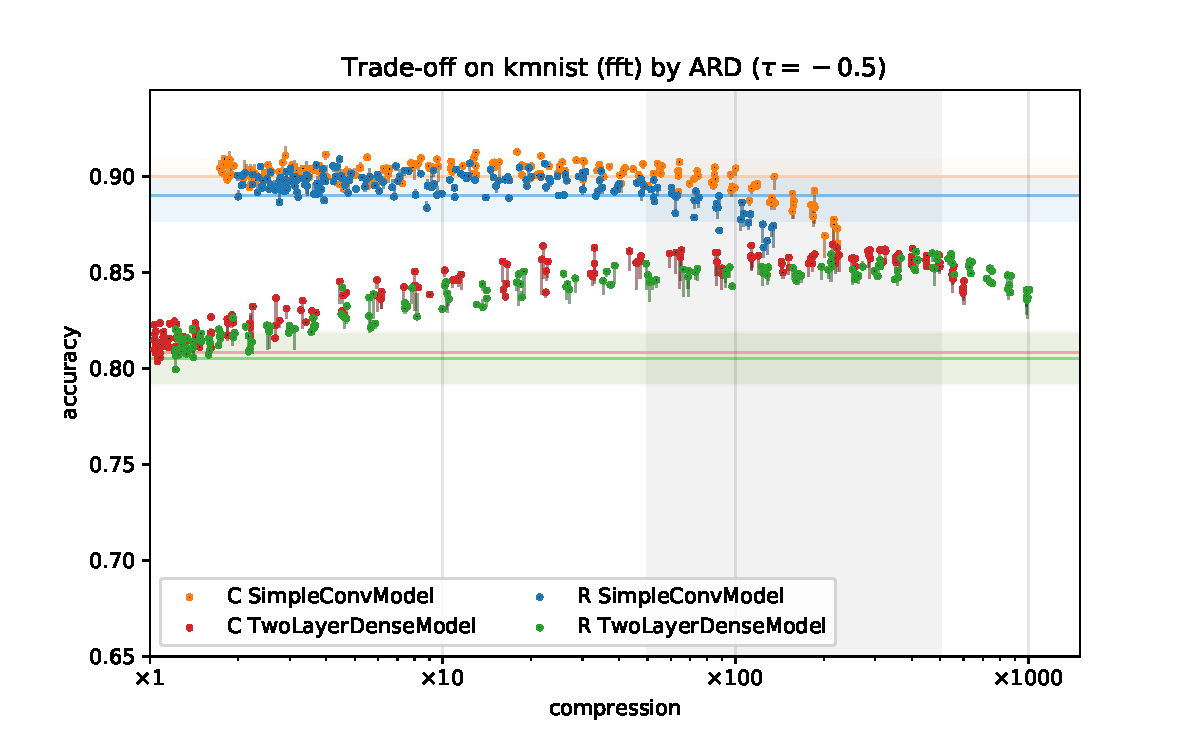
\includegraphics[width=\linewidth]{figure__mnist-like__trade-off/appendix__ARD__kmnist__fft__-0.5.pdf}
  \end{subfigure} \\ %
  \begin{subfigure}[b]{0.5\columnwidth}
    \centering
    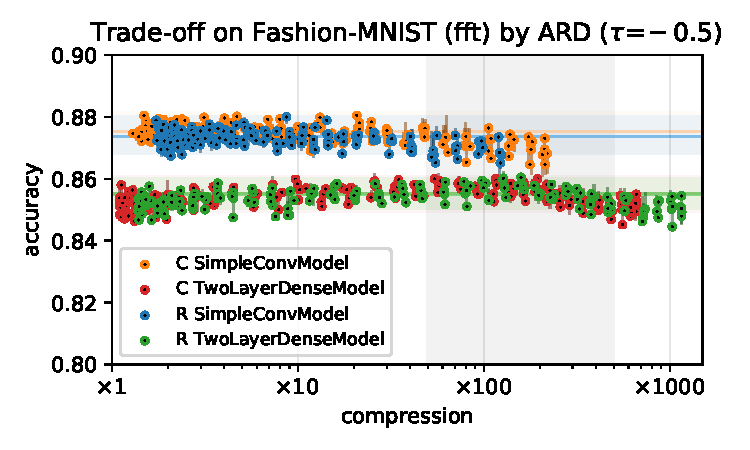
\includegraphics[width=\linewidth]{figure__mnist-like__trade-off/appendix__ARD__fashionmnist__fft__-0.5.pdf}
  \end{subfigure}%
  \begin{subfigure}[b]{0.5\columnwidth}
    \centering
    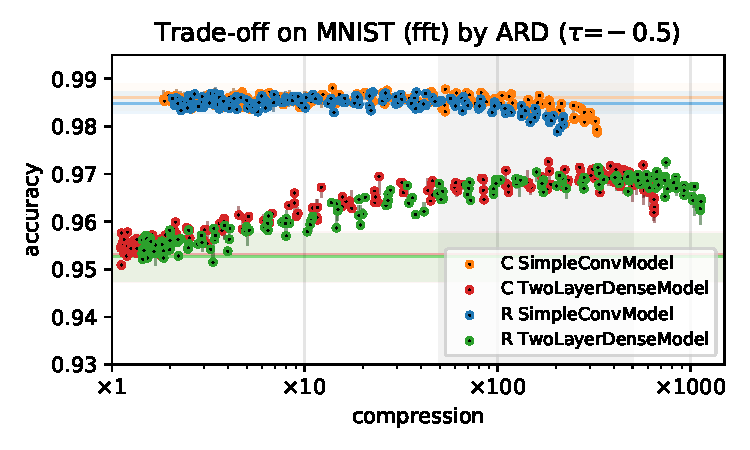
\includegraphics[width=\linewidth]{figure__mnist-like__trade-off/appendix__ARD__mnist__fft__-0.5.pdf}
  \end{subfigure}
  \caption{%
    The trade-off of ARD method for $\real$ and $\cplx$ models using Fourier features.
  }
  \label{fig:appendix__mnist-like__trade-off__ARD__fft}
\end{figure}

\begin{figure}[b]
  \centering
  \begin{subfigure}[b]{0.5\columnwidth}
    \centering
    % used in main text
    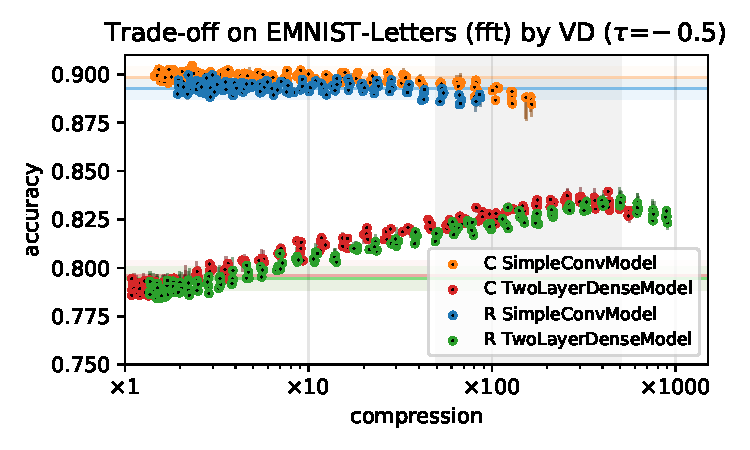
\includegraphics[width=\linewidth]{figure__mnist-like__trade-off/appendix__VD__emnist_letters__fft__-0.5.pdf}
  \end{subfigure}%
  \begin{subfigure}[b]{0.5\columnwidth}
    \centering
    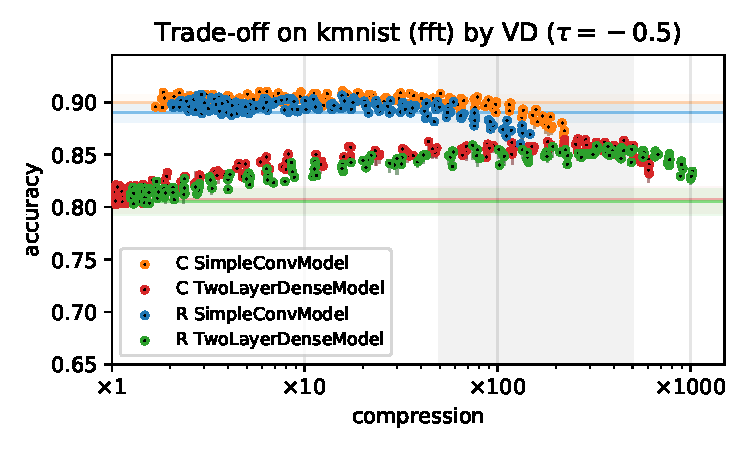
\includegraphics[width=\linewidth]{figure__mnist-like__trade-off/appendix__VD__kmnist__fft__-0.5.pdf}
  \end{subfigure} \\ %
  \begin{subfigure}[b]{0.5\columnwidth}
    \centering
    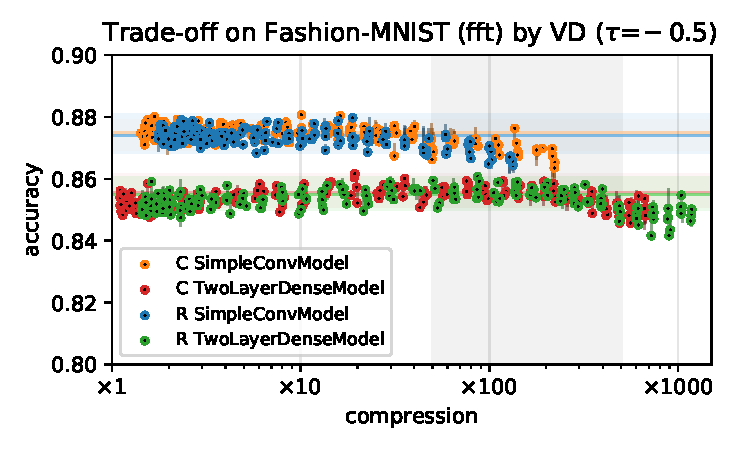
\includegraphics[width=\linewidth]{figure__mnist-like__trade-off/appendix__VD__fashionmnist__fft__-0.5.pdf}
  \end{subfigure}%
  \begin{subfigure}[b]{0.5\columnwidth}
    \centering
    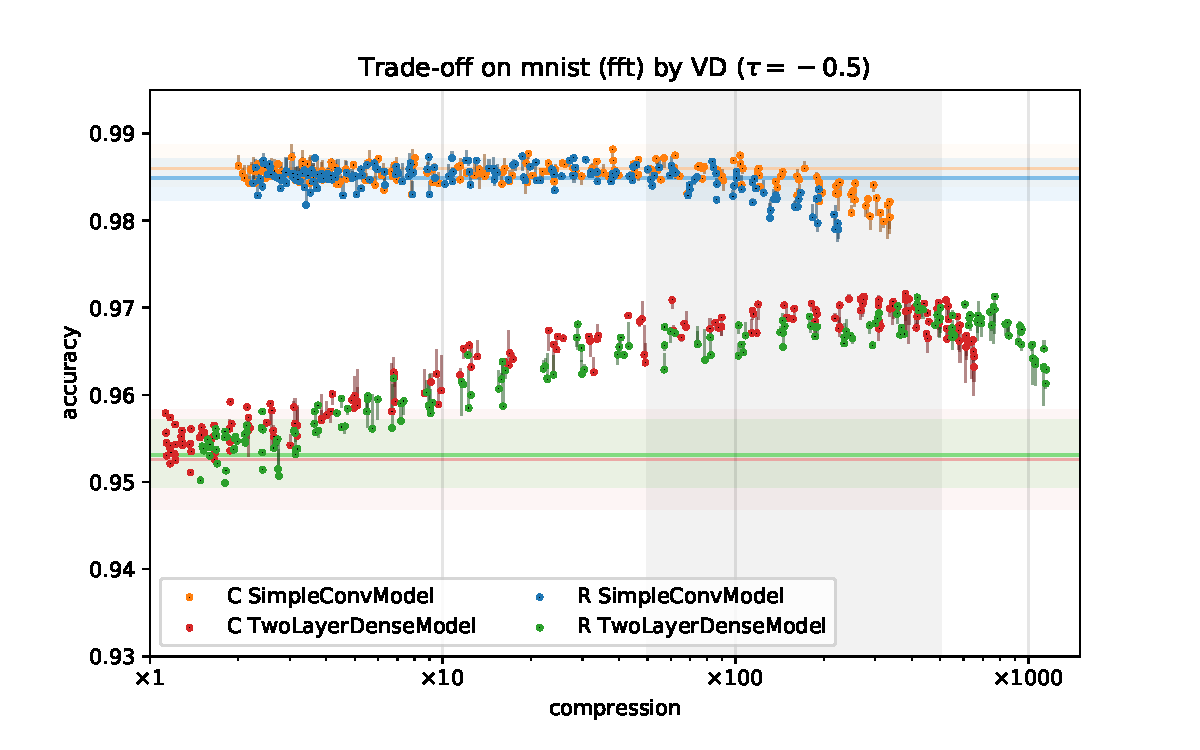
\includegraphics[width=\linewidth]{figure__mnist-like__trade-off/appendix__VD__mnist__fft__-0.5.pdf}
  \end{subfigure}
  \caption{%
    The trade-off of VD method for $\real$ and $\cplx$ models using Fourier features.
  }
  \label{fig:appendix__mnist-like__trade-off__VD__fft}
\end{figure}

\begin{figure}[b]
  \centering
  \begin{subfigure}[b]{0.5\columnwidth}
    \centering
    % used in main text
    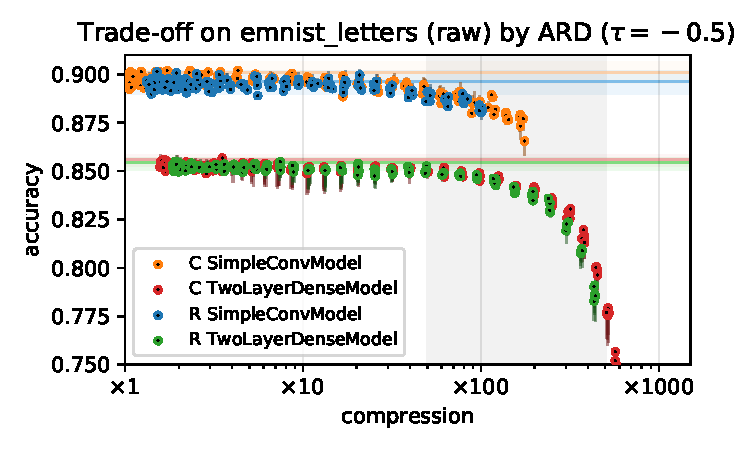
\includegraphics[width=\linewidth]{figure__mnist-like__trade-off/appendix__ARD__emnist_letters__raw__-0.5.pdf}
  \end{subfigure}%
  \begin{subfigure}[b]{0.5\columnwidth}
    \centering
    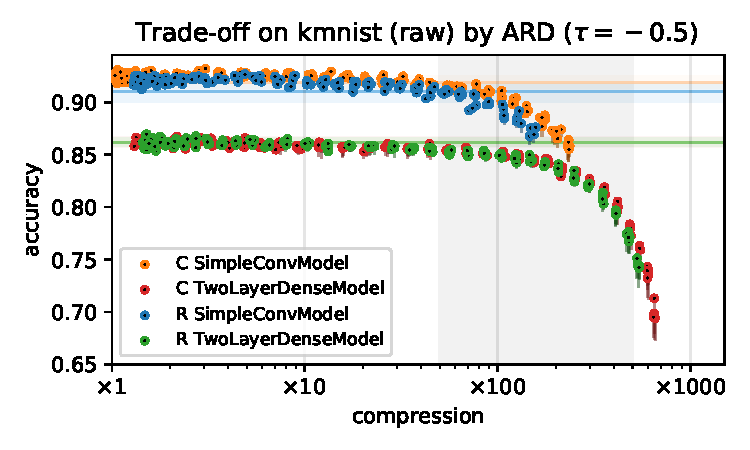
\includegraphics[width=\linewidth]{figure__mnist-like__trade-off/appendix__ARD__kmnist__raw__-0.5.pdf}
  \end{subfigure} \\%
  \begin{subfigure}[b]{0.5\columnwidth}
    \centering
    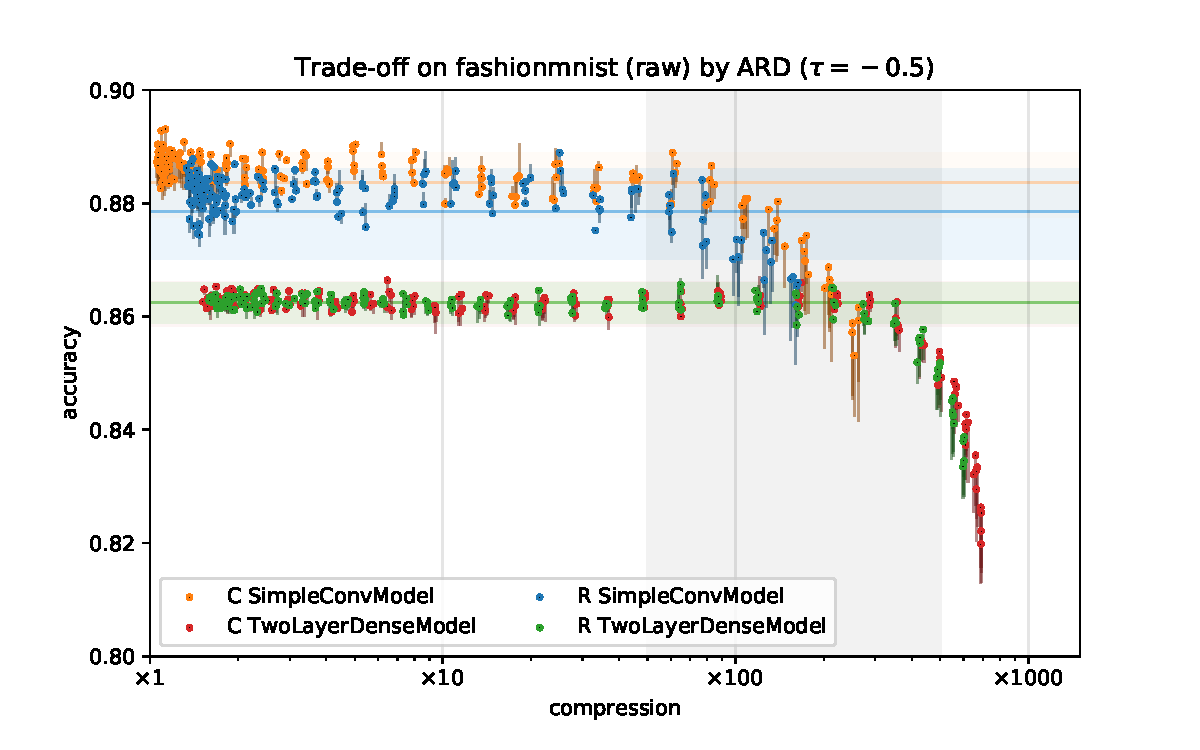
\includegraphics[width=\linewidth]{figure__mnist-like__trade-off/appendix__ARD__fashionmnist__raw__-0.5.pdf}
  \end{subfigure}%
  \begin{subfigure}[b]{0.5\columnwidth}
    \centering
    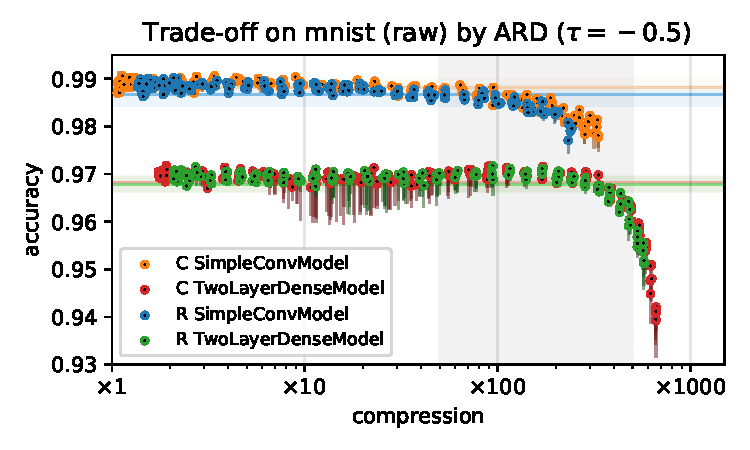
\includegraphics[width=\linewidth]{figure__mnist-like__trade-off/appendix__ARD__mnist__raw__-0.5.pdf}
  \end{subfigure}
  \caption{%
    The trade-off of ARD method for $\real$ and $\cplx$ models using raw features.
  }
  \label{fig:appendix__mnist-like__trade-off__ARD__raw}
\end{figure}

\begin{figure}[b]
  \centering
  \begin{subfigure}[b]{0.5\columnwidth}
    \centering
    % used in main text
    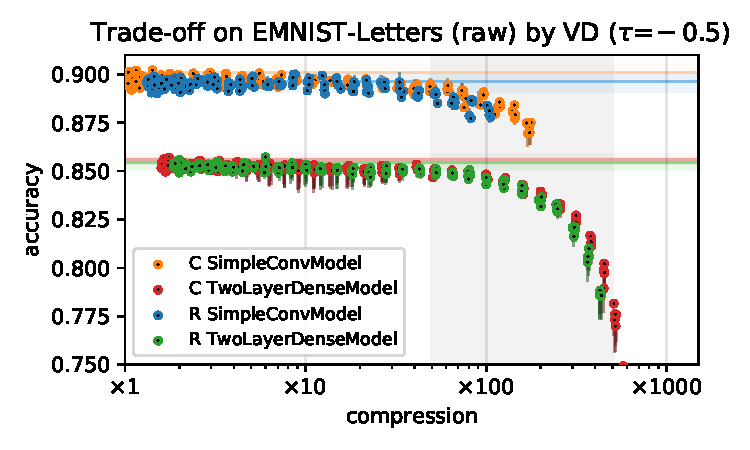
\includegraphics[width=\linewidth]{figure__mnist-like__trade-off/appendix__VD__emnist_letters__raw__-0.5.pdf}
  \end{subfigure}%
  \begin{subfigure}[b]{0.5\columnwidth}
    \centering
    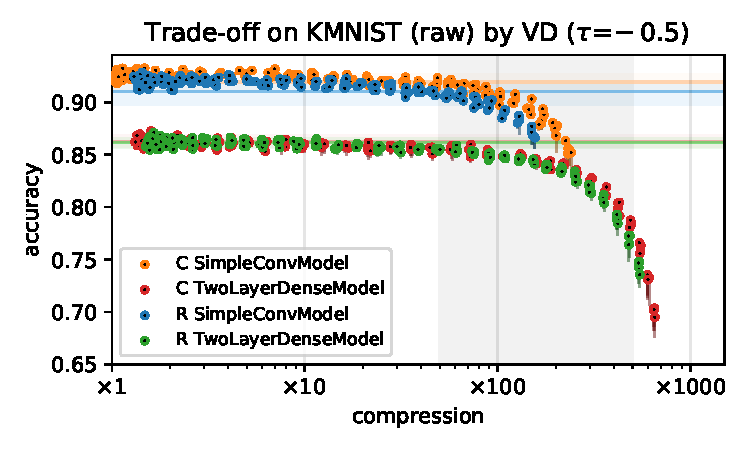
\includegraphics[width=\linewidth]{figure__mnist-like__trade-off/appendix__VD__kmnist__raw__-0.5.pdf}
  \end{subfigure} \\%
  \begin{subfigure}[b]{0.5\columnwidth}
    \centering
    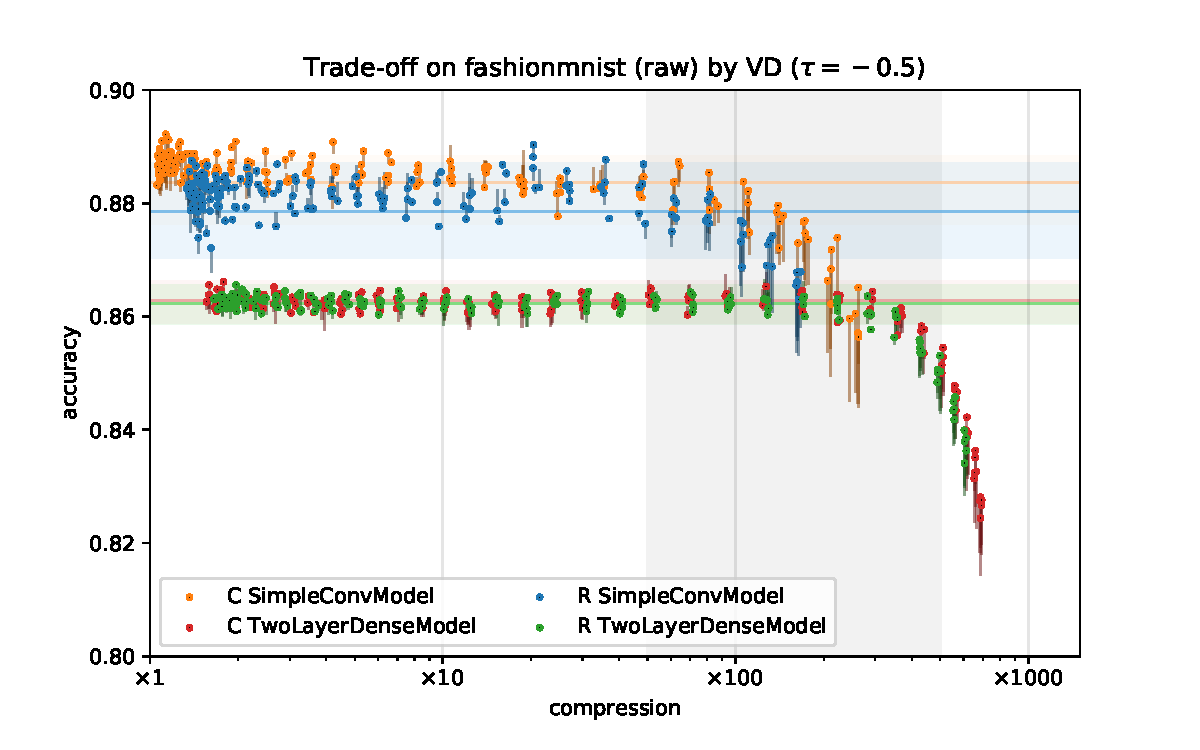
\includegraphics[width=\linewidth]{figure__mnist-like__trade-off/appendix__VD__fashionmnist__raw__-0.5.pdf}
  \end{subfigure}%
  \begin{subfigure}[b]{0.5\columnwidth}
    \centering
    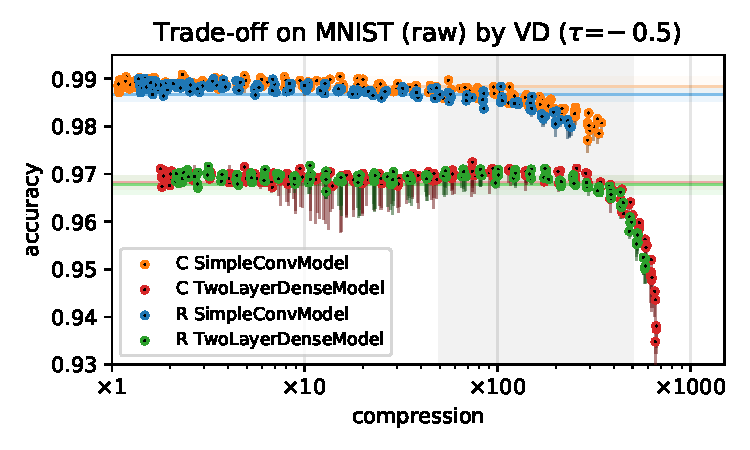
\includegraphics[width=\linewidth]{figure__mnist-like__trade-off/appendix__VD__mnist__raw__-0.5.pdf}
  \end{subfigure}
  \caption{%
    The trade-off of VD method for $\real$ and $\cplx$ models using raw features.
  }
  \label{fig:appendix__mnist-like__trade-off__VD__raw}
\end{figure}

\begin{figure}[b]
  \centering
  \begin{subfigure}[b]{0.5\columnwidth}
    \centering
    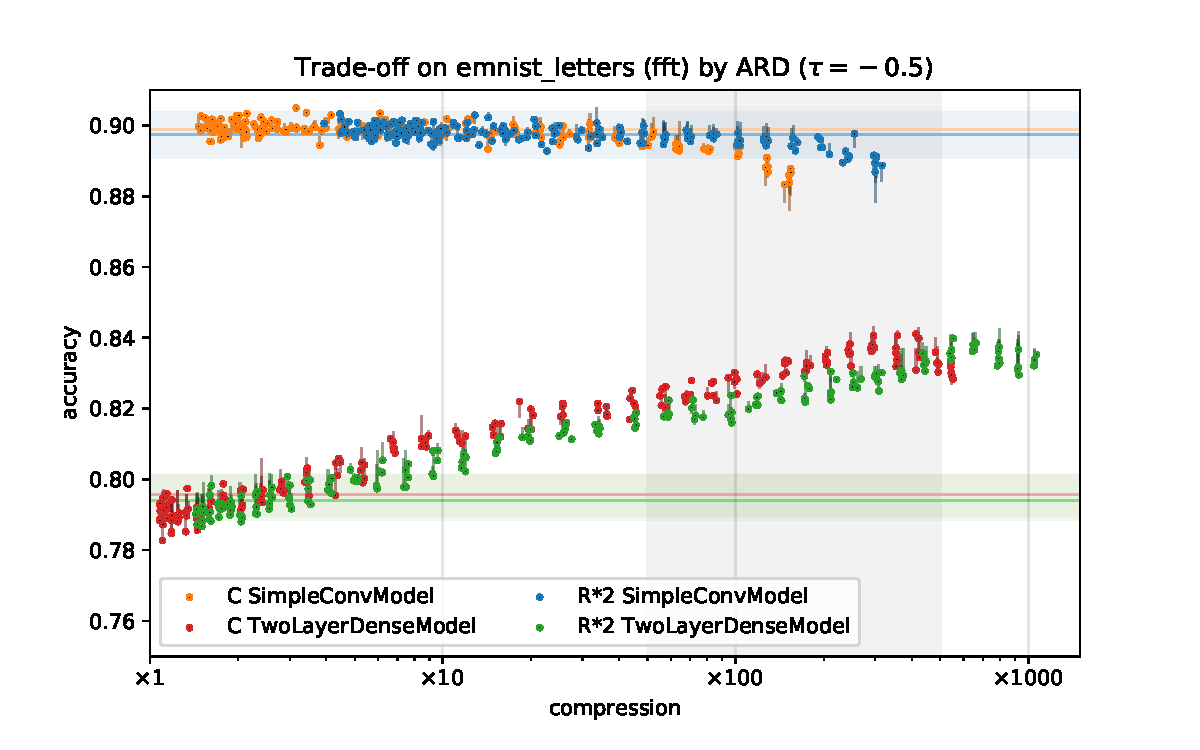
\includegraphics[width=\linewidth]{figure__mnist-like__trade-off/appendix__cmp__ARD__emnist_letters__fft__-0.5.pdf}
  \end{subfigure}%
  \begin{subfigure}[b]{0.5\columnwidth}
    \centering
    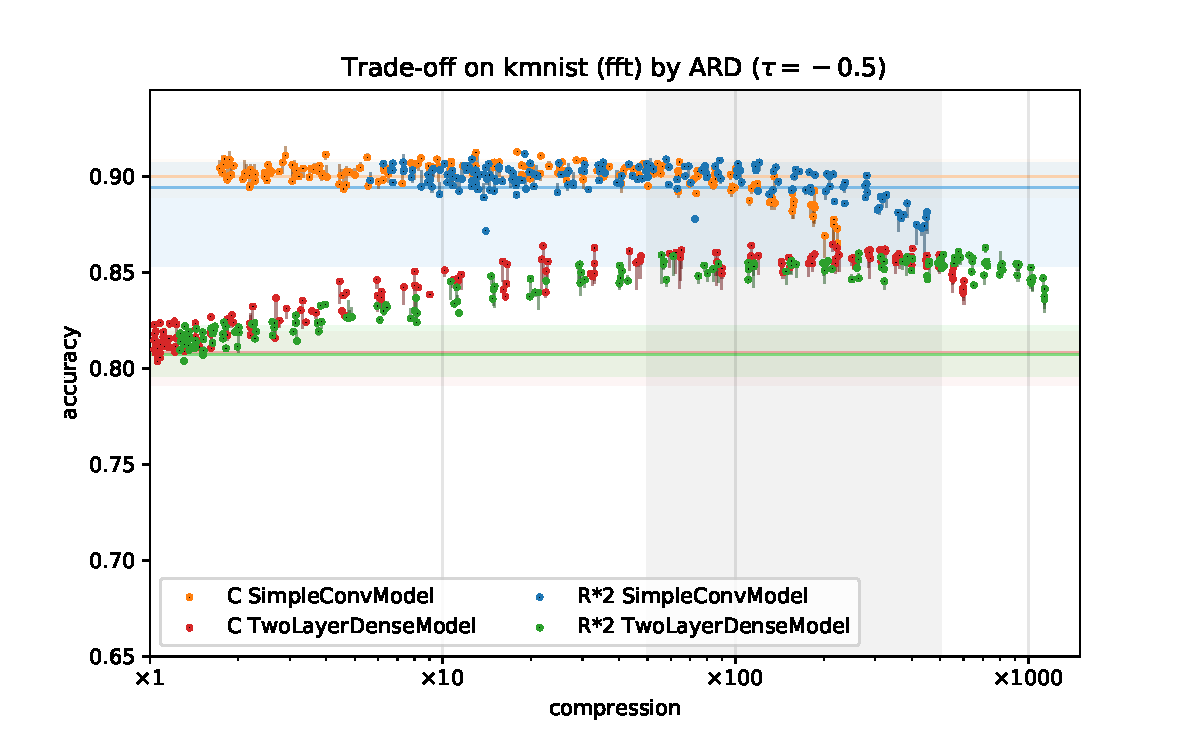
\includegraphics[width=\linewidth]{figure__mnist-like__trade-off/appendix__cmp__ARD__kmnist__fft__-0.5.pdf}
  \end{subfigure} \\ %
  \begin{subfigure}[b]{0.5\columnwidth}
    \centering
    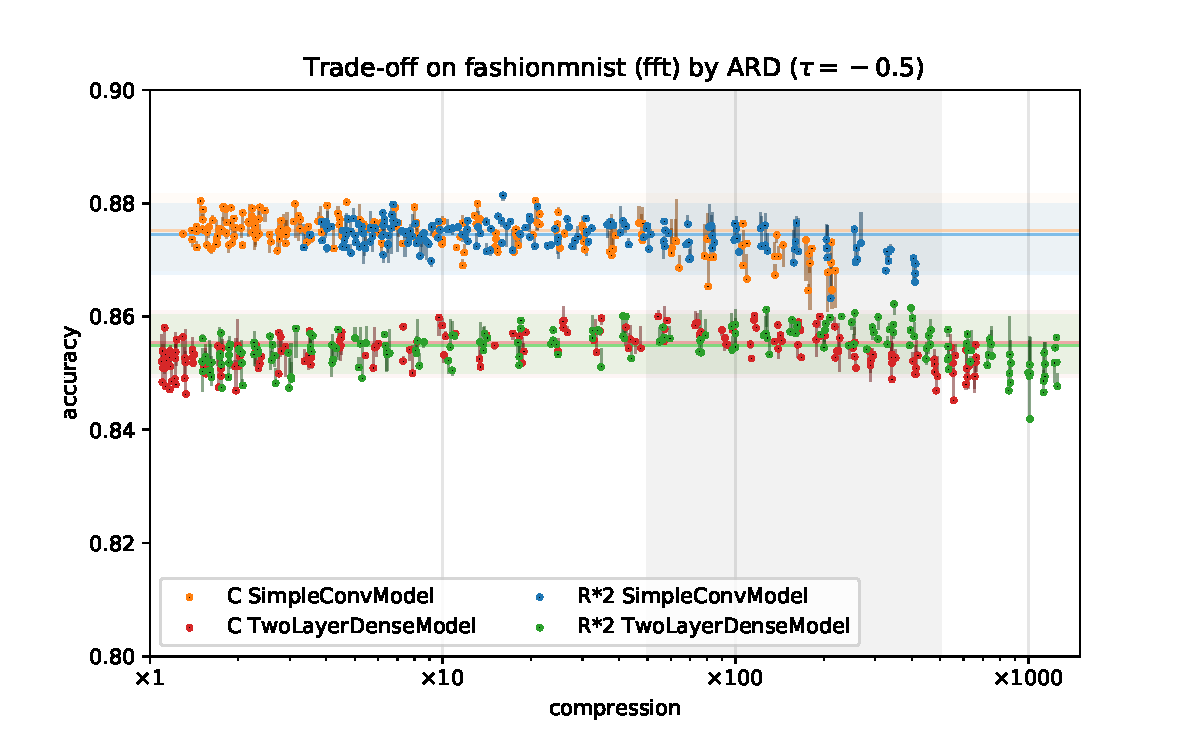
\includegraphics[width=\linewidth]{figure__mnist-like__trade-off/appendix__cmp__ARD__fashionmnist__fft__-0.5.pdf}
  \end{subfigure}%
  \begin{subfigure}[b]{0.5\columnwidth}
    \centering
    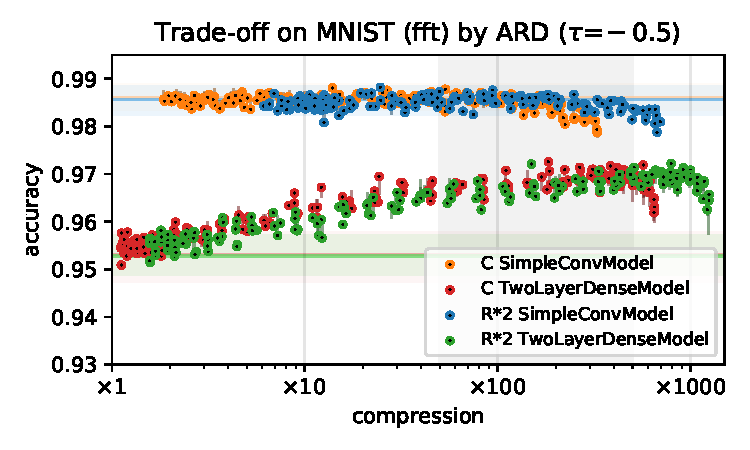
\includegraphics[width=\linewidth]{figure__mnist-like__trade-off/appendix__cmp__ARD__mnist__fft__-0.5.pdf}
  \end{subfigure}
  \caption{%
    The trade-off of ARD method for $2\real$ and $\cplx$ models using Fourier features.
  }
  \label{fig:appendix__cmp__mnist-like__trade-off__ARD__fft}
\end{figure}

\begin{figure}[b]
  \centering
  \begin{subfigure}[b]{0.5\columnwidth}
    \centering
    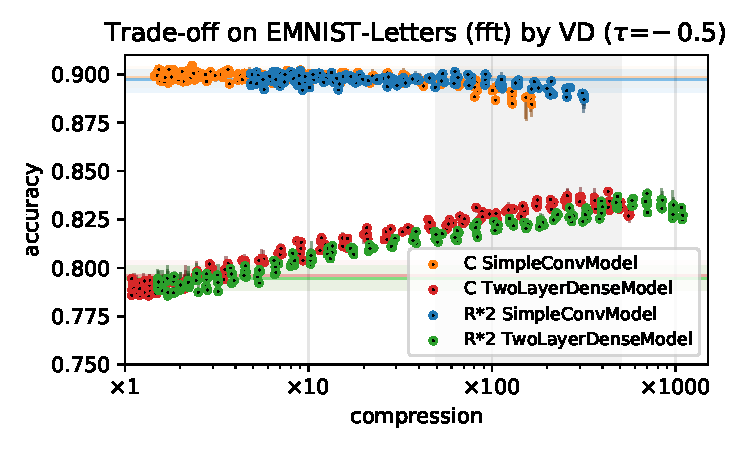
\includegraphics[width=\linewidth]{figure__mnist-like__trade-off/appendix__cmp__VD__emnist_letters__fft__-0.5.pdf}
  \end{subfigure}%
  \begin{subfigure}[b]{0.5\columnwidth}
    \centering
    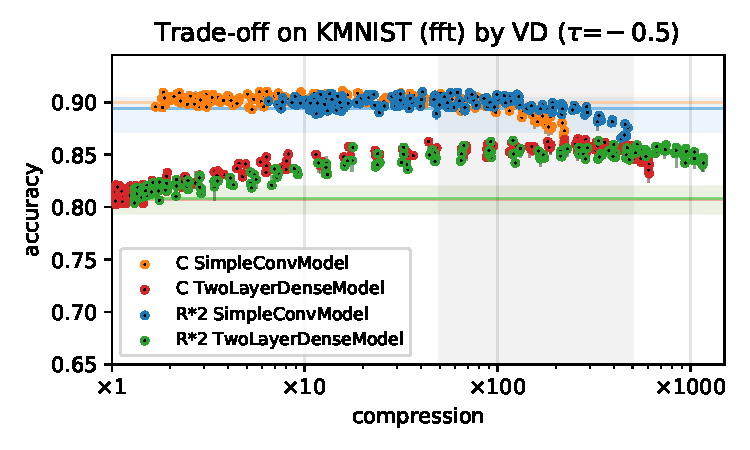
\includegraphics[width=\linewidth]{figure__mnist-like__trade-off/appendix__cmp__VD__kmnist__fft__-0.5.pdf}
  \end{subfigure} \\ %
  \begin{subfigure}[b]{0.5\columnwidth}
    \centering
    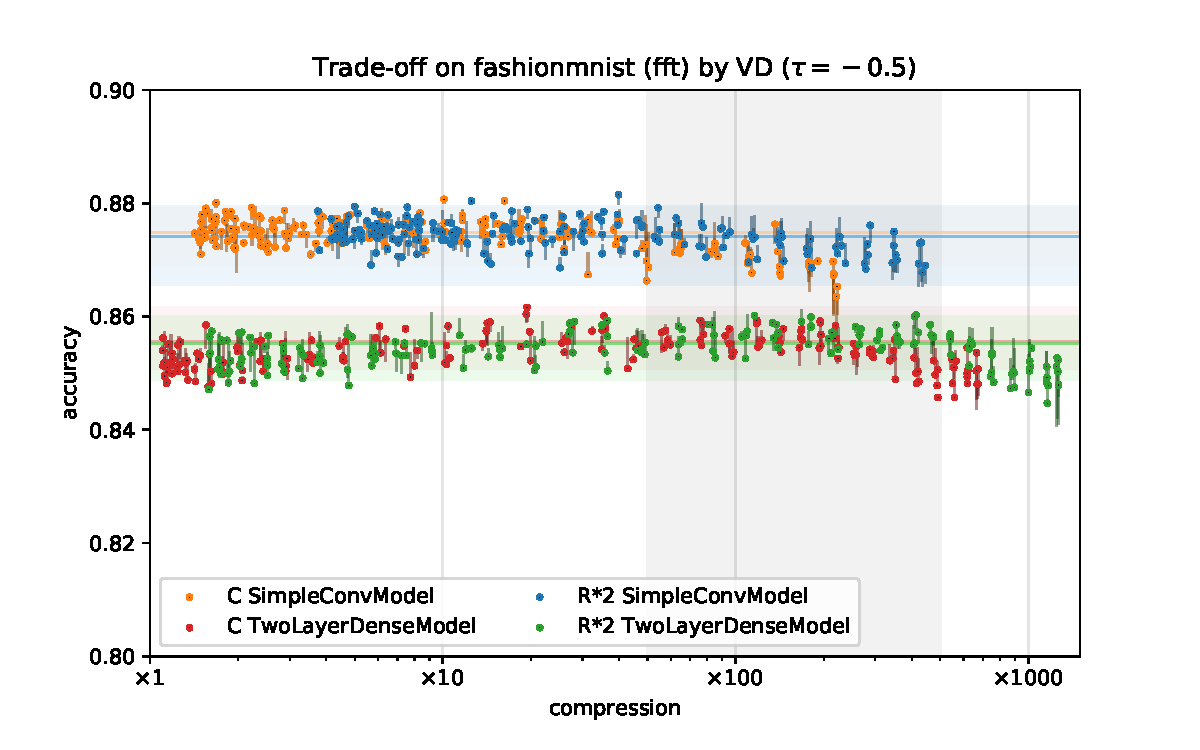
\includegraphics[width=\linewidth]{figure__mnist-like__trade-off/appendix__cmp__VD__fashionmnist__fft__-0.5.pdf}
  \end{subfigure}%
  \begin{subfigure}[b]{0.5\columnwidth}
    \centering
    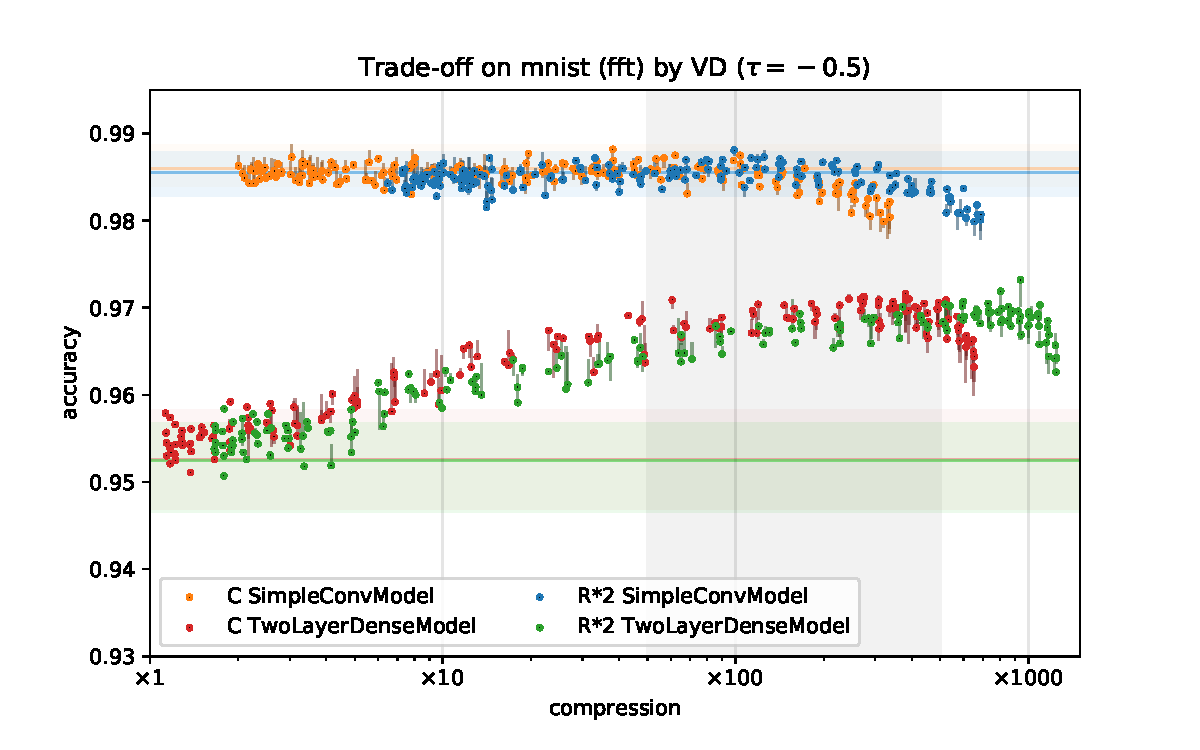
\includegraphics[width=\linewidth]{figure__mnist-like__trade-off/appendix__cmp__VD__mnist__fft__-0.5.pdf}
  \end{subfigure}
  \caption{%
    The trade-off of VD method for $2\real$ and $\cplx$ models using Fourier features.
  }
  \label{fig:appendix__cmp__mnist-like__trade-off__VD__fft}
\end{figure}

\begin{figure}[b]
  \centering
  \begin{subfigure}[b]{0.5\columnwidth}
    \centering
    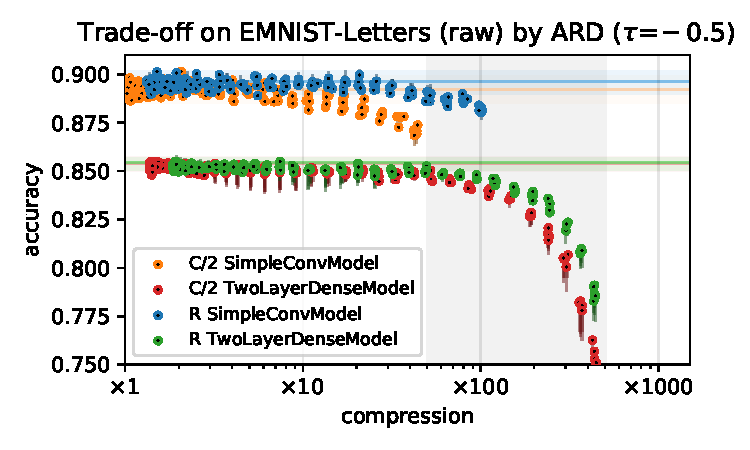
\includegraphics[width=\linewidth]{figure__mnist-like__trade-off/appendix__cmp__ARD__emnist_letters__raw__-0.5.pdf}
  \end{subfigure}%
  \begin{subfigure}[b]{0.5\columnwidth}
    \centering
    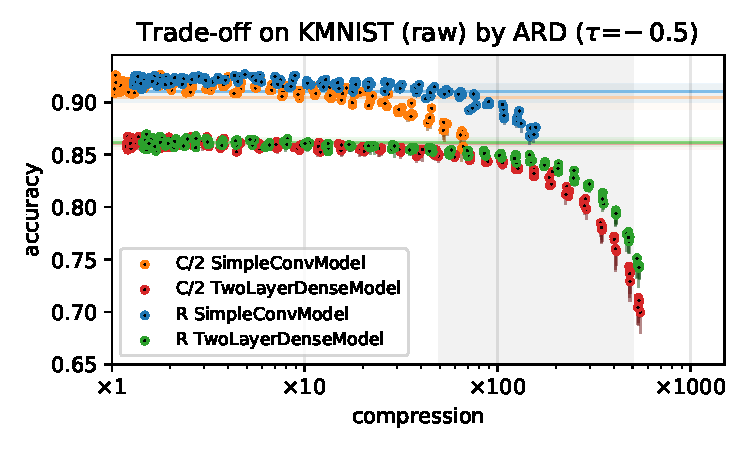
\includegraphics[width=\linewidth]{figure__mnist-like__trade-off/appendix__cmp__ARD__kmnist__raw__-0.5.pdf}
  \end{subfigure} \\%
  \begin{subfigure}[b]{0.5\columnwidth}
    \centering
    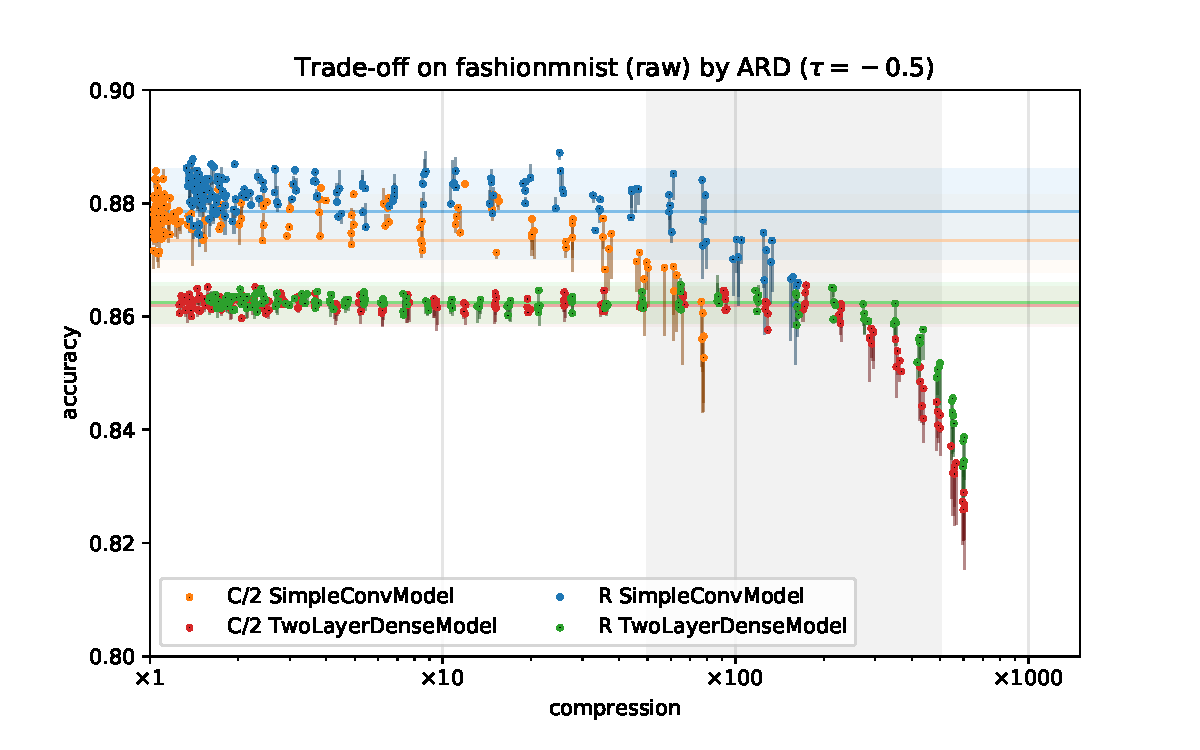
\includegraphics[width=\linewidth]{figure__mnist-like__trade-off/appendix__cmp__ARD__fashionmnist__raw__-0.5.pdf}
  \end{subfigure}%
  \begin{subfigure}[b]{0.5\columnwidth}
    \centering
    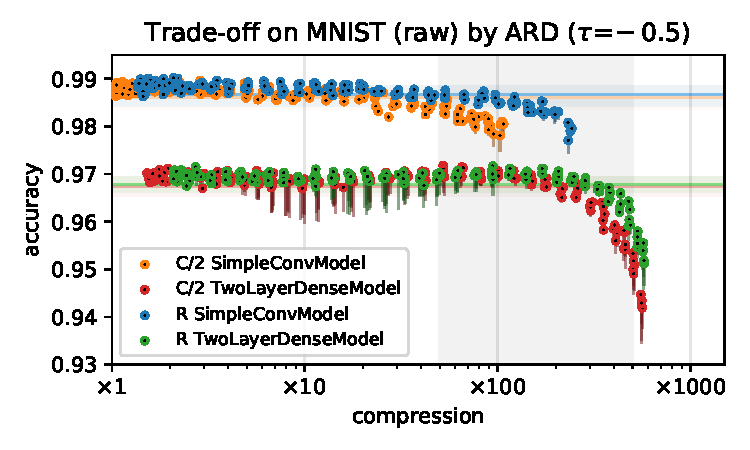
\includegraphics[width=\linewidth]{figure__mnist-like__trade-off/appendix__cmp__ARD__mnist__raw__-0.5.pdf}
  \end{subfigure}
  \caption{%
    The trade-off of ARD method for $\real$ and $\tfrac12\cplx$ models using raw features.
  }
  \label{fig:appendix__cmp__mnist-like__trade-off__ARD__raw}
\end{figure}

\begin{figure}[b]
  \centering
  \begin{subfigure}[b]{0.5\columnwidth}
    \centering
    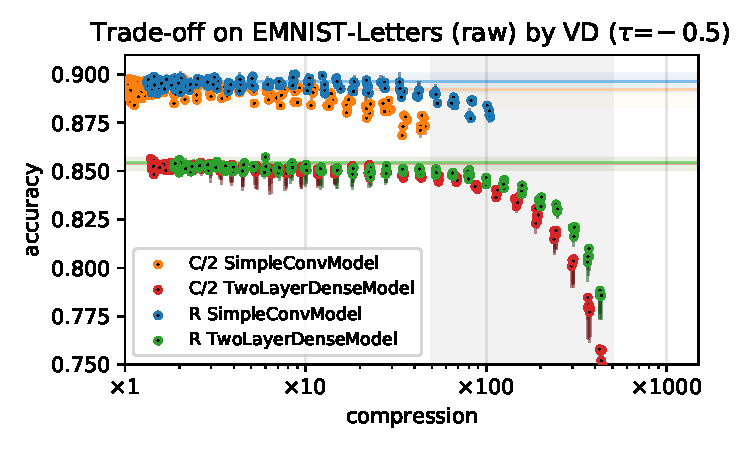
\includegraphics[width=\linewidth]{figure__mnist-like__trade-off/appendix__cmp__VD__emnist_letters__raw__-0.5.pdf}
  \end{subfigure}%
  \begin{subfigure}[b]{0.5\columnwidth}
    \centering
    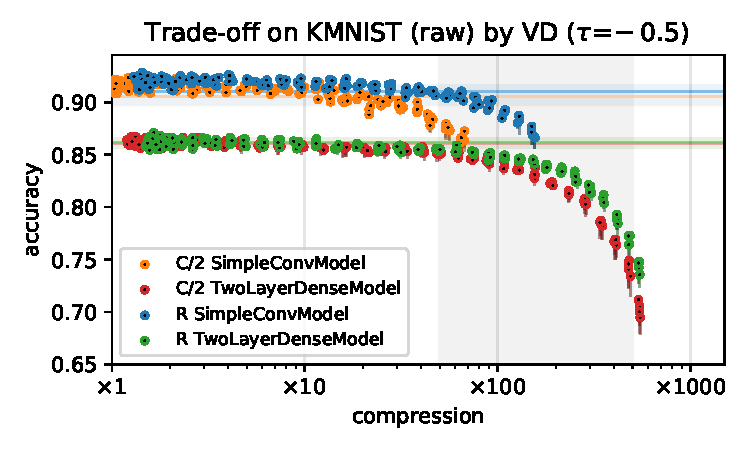
\includegraphics[width=\linewidth]{figure__mnist-like__trade-off/appendix__cmp__VD__kmnist__raw__-0.5.pdf}
  \end{subfigure} \\%
  \begin{subfigure}[b]{0.5\columnwidth}
    \centering
    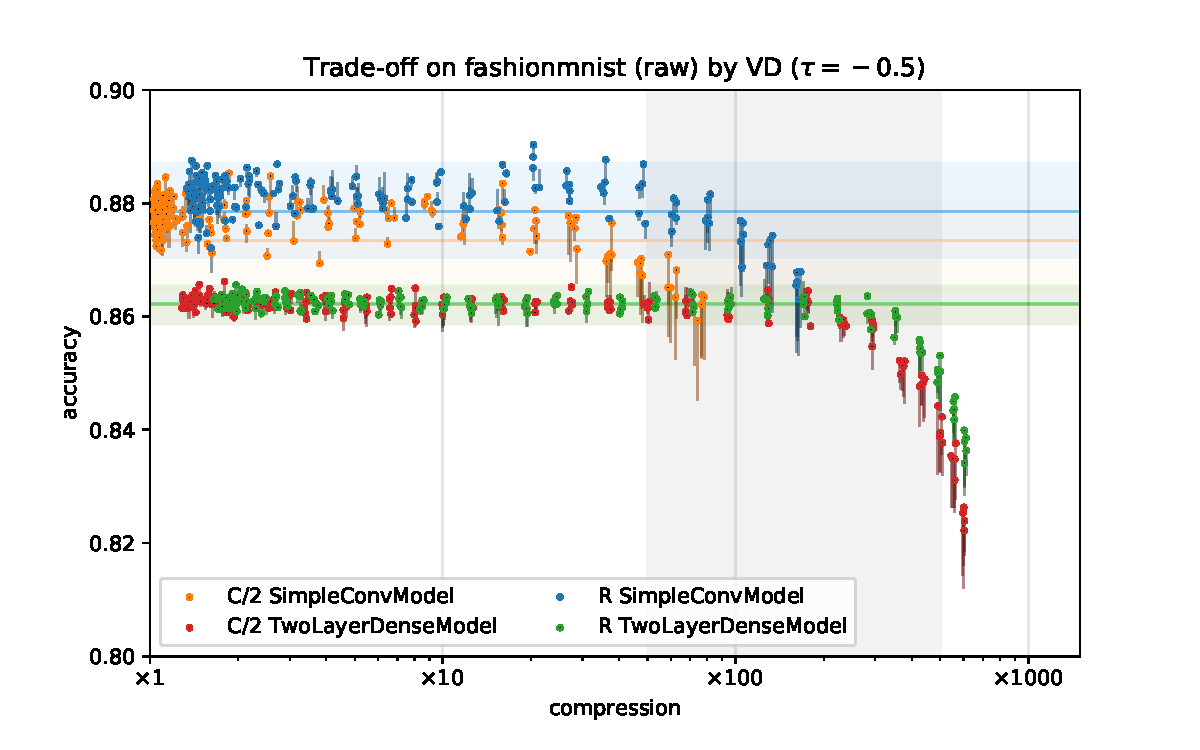
\includegraphics[width=\linewidth]{figure__mnist-like__trade-off/appendix__cmp__VD__fashionmnist__raw__-0.5.pdf}
  \end{subfigure}%
  \begin{subfigure}[b]{0.5\columnwidth}
    \centering
    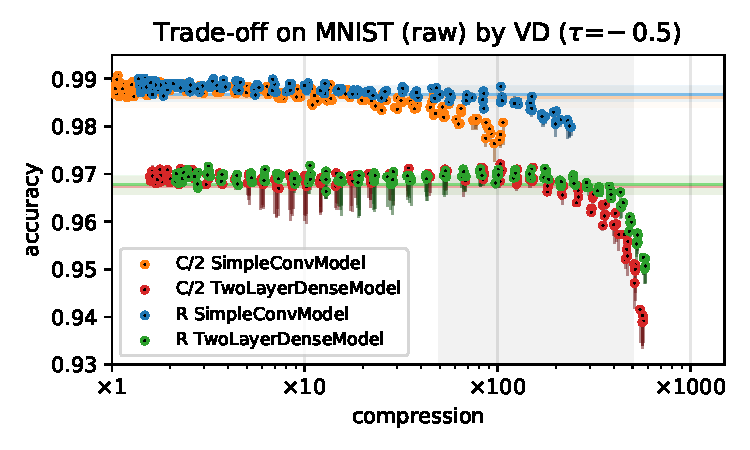
\includegraphics[width=\linewidth]{figure__mnist-like__trade-off/appendix__cmp__VD__mnist__raw__-0.5.pdf}
  \end{subfigure}
  \caption{%
    The trade-off of VD method for $\real$ and $\tfrac12\cplx$ models using raw features.
  }
  \label{fig:appendix__cmp__mnist-like__trade-off__VD__raw}
\end{figure}

\begin{figure}[b]
  \centering
  \begin{subfigure}[b]{0.5\columnwidth}
    \centering
    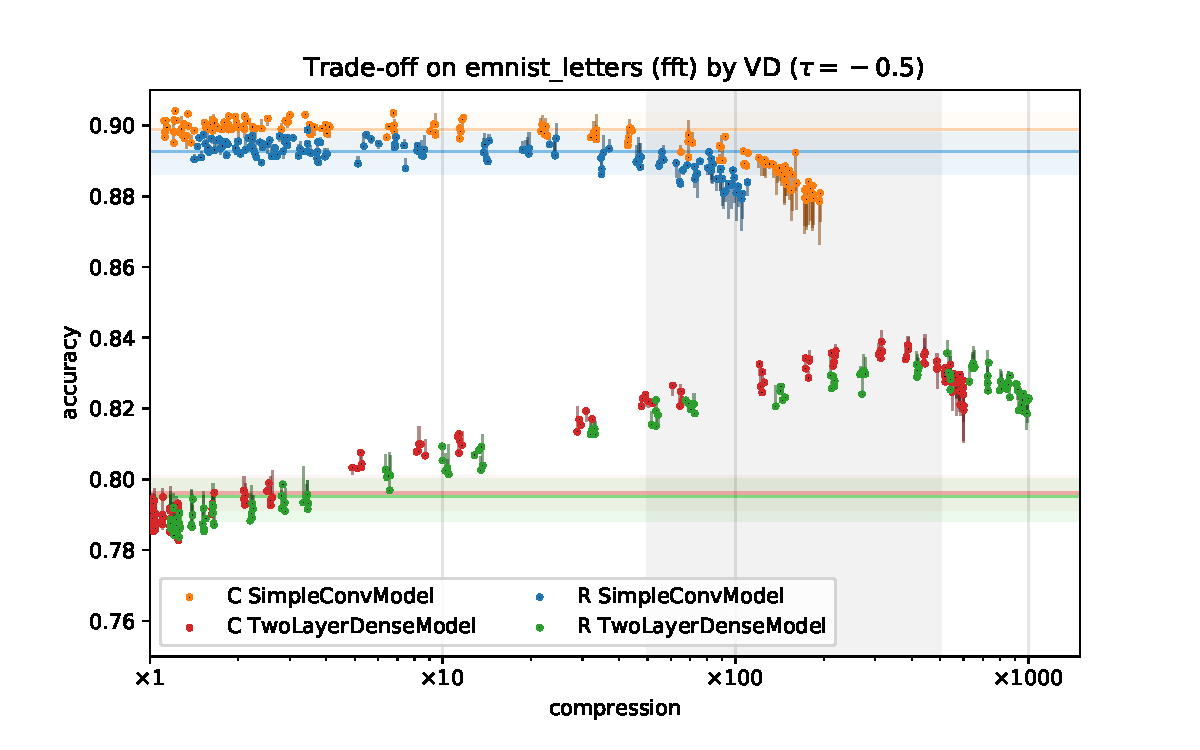
\includegraphics[width=\linewidth]{figure__mnist-like__trade-off/legacy__VD__emnist_letters__fft__-0.5.pdf}
  \end{subfigure}%
  \begin{subfigure}[b]{0.5\columnwidth}
    \centering
    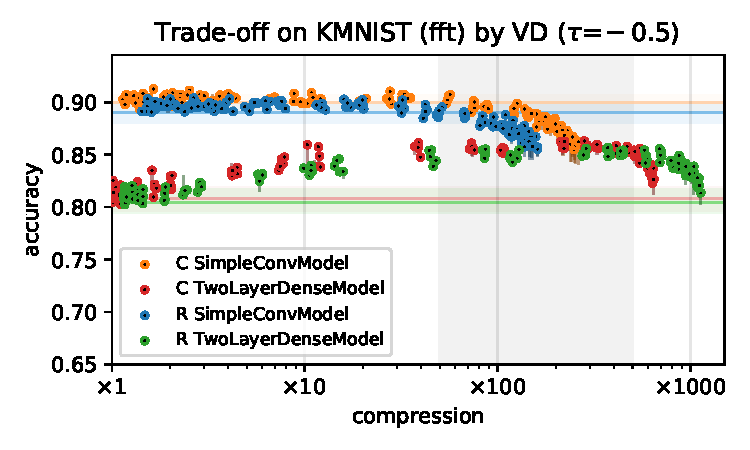
\includegraphics[width=\linewidth]{figure__mnist-like__trade-off/legacy__VD__kmnist__fft__-0.5.pdf}
  \end{subfigure} \\%
  \begin{subfigure}[b]{0.5\columnwidth}
    \centering
    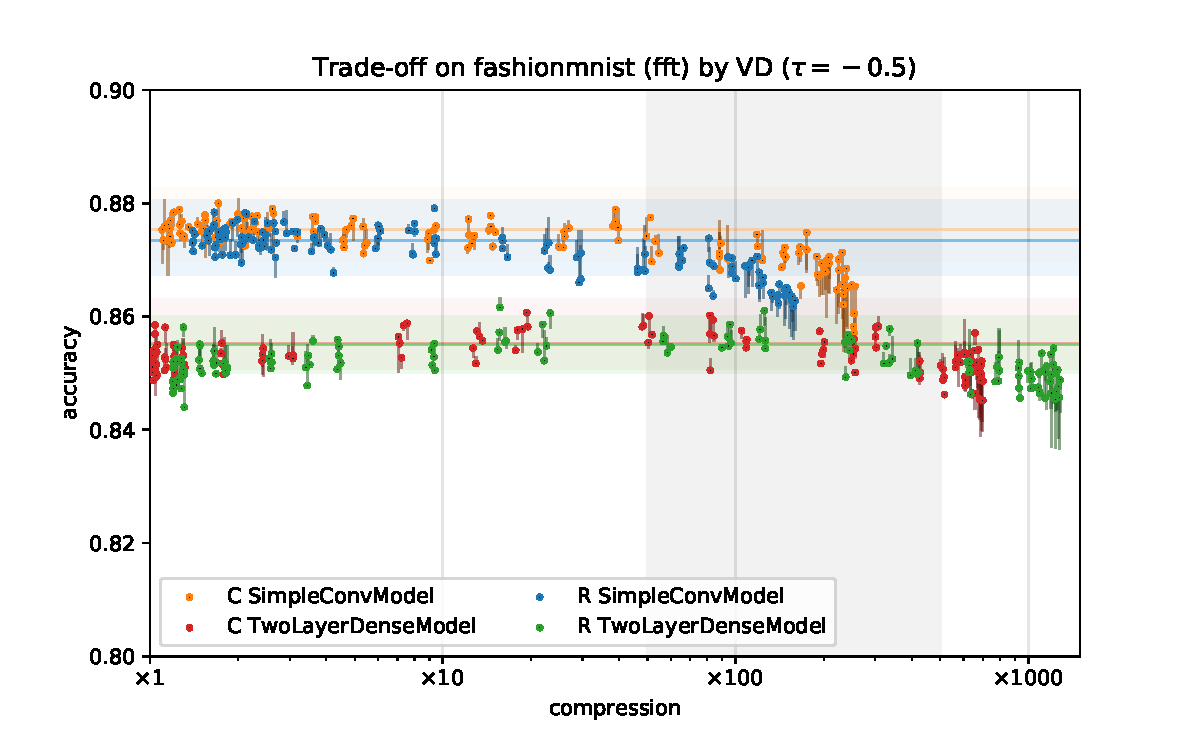
\includegraphics[width=\linewidth]{figure__mnist-like__trade-off/legacy__VD__fashionmnist__fft__-0.5.pdf}
  \end{subfigure}%
  \begin{subfigure}[b]{0.5\columnwidth}
    \centering
    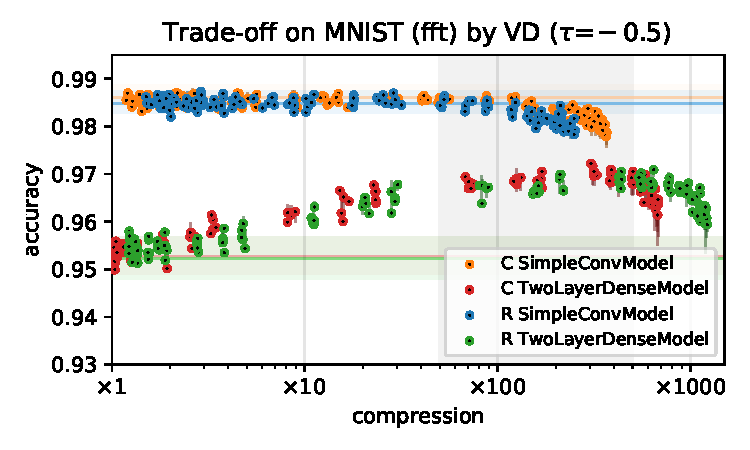
\includegraphics[width=\linewidth]{figure__mnist-like__trade-off/legacy__VD__mnist__fft__-0.5.pdf}
  \end{subfigure}
  \caption{%
    The trade-off of VD method for $\real$ and $\cplx$ models using Fourier features (main text).
  }
  \label{fig:paper__mnist-like__trade-off__VD__fft}
\end{figure}

\begin{figure}[b]
  \centering
  \begin{subfigure}[b]{0.5\columnwidth}
    \centering
    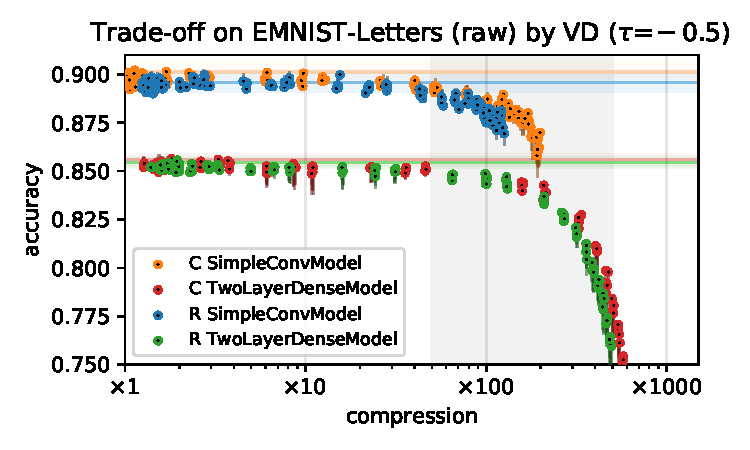
\includegraphics[width=\linewidth]{figure__mnist-like__trade-off/legacy__VD__emnist_letters__raw__-0.5.pdf}
  \end{subfigure}%
  \begin{subfigure}[b]{0.5\columnwidth}
    \centering
    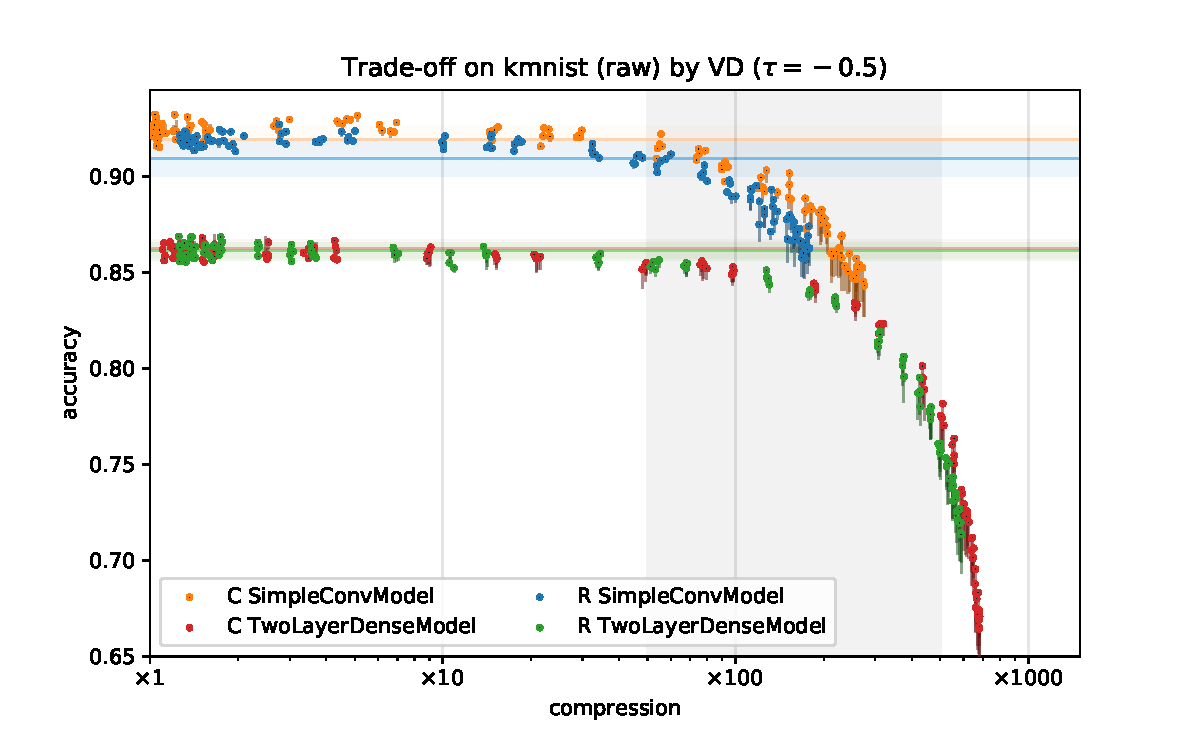
\includegraphics[width=\linewidth]{figure__mnist-like__trade-off/legacy__VD__kmnist__raw__-0.5.pdf}
  \end{subfigure} \\%
  \begin{subfigure}[b]{0.5\columnwidth}
    \centering
    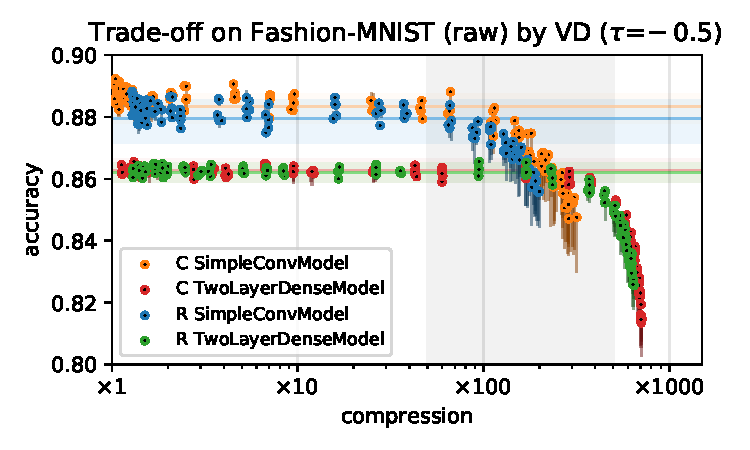
\includegraphics[width=\linewidth]{figure__mnist-like__trade-off/legacy__VD__fashionmnist__raw__-0.5.pdf}
  \end{subfigure}%
  \begin{subfigure}[b]{0.5\columnwidth}
    \centering
    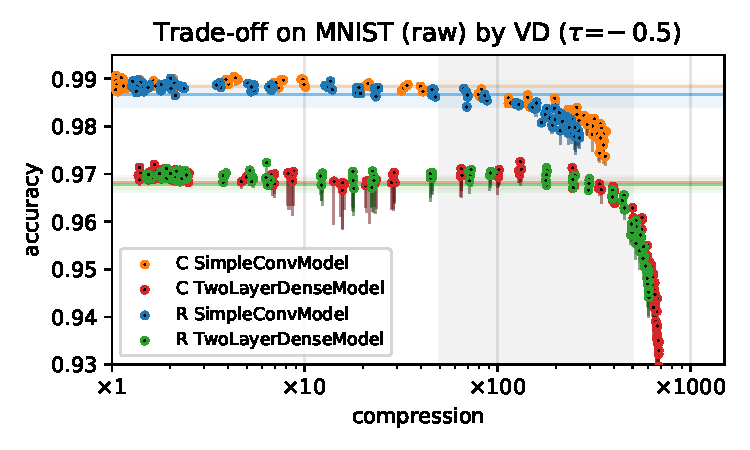
\includegraphics[width=\linewidth]{figure__mnist-like__trade-off/legacy__VD__mnist__raw__-0.5.pdf}
  \end{subfigure}
  \caption{%
    The trade-off of VD method for $\real$ and $\cplx$ models using raw features (main text).
  }
  \label{fig:paper__mnist-like__trade-off__VD__raw}
\end{figure}

% \clearpage

% section mnist_like_experiments (end)

\section{Complex-valued local reparameterization} % (fold)
\label{sec:complex_valued_local_reparameterization}

%notation
By $e_i$ we denote the $i$-th real unit vector of dimensionality \emph{conforming} to the
matrix-vector expression it is used in. Let $\vec{M}$ denote \emph{row-major} flattening
of $M$ into a vector, i.e. in lexicographic order of its indices. $\diag{(\cdot)}$ embeds
$\cplx^n$ into $n\times n$ diagonal matrices, and $\otimes$ denotes the Kronecker product,
for which we note the following identities $
  \vec{P Q R} = (P \otimes R^\top) \vec{Q}
$, and $
  (P \otimes R) (C \otimes S) = P Q \otimes R S
$ \citep{petersen_matrix_2012}.
% It follows from the definition of the Kronecker product
% of $P$ and $R^\top$ and the row-major order vectorization.

If we assume a mean field $\cplx$-Gaussian approximate posterior for $
  W \in \cplx^{n\times m}
$, then
\begin{equation}  \label{eq:c-gauss-vi-general-vec}
  \vec{W}
    \sim \mathcal{N}^{\cplx}_{nm} \bigl(
      \vec{\mu}, \diag{\vec{\Sigma}}, \diag{\vec{C}}
    \bigr)
  \,,
\end{equation}
where mean, \emph{variance} and relation are given by matrices $
  \mu, \Sigma, C \in \cplx^{n\times m}
$ with $\Sigma_{ij} \geq 0$, and $
  \lvert C_{ij} \rvert^2 \leq \Sigma_{ij}
$. For any $x \in \cplx^m$ and $b\in \cplx^n$ $
  y = W x + b
    = (I_n \otimes x^\top) \vec{W} + b
$, whence the covariance and relation matrices of $y$ are
\begin{align}
  (I \otimes x^\top) \diag{\vec{\Sigma}} (I \otimes x^\top)^{\hop}
    % = \sum_{ij} (I \otimes x^\top) e_i \otimes e_j
    %   \Sigma_{ij} (e_i \otimes e_j)^\top (I \otimes x^\top)^{\hop}
    % = \sum_{ij} (e_i \otimes x^\top e_j)
    %   \Sigma_{ij} (e_i \otimes x^\top e_j)^{\hop}
    % = \sum_{ij} (e_i \otimes x_j) \Sigma_{ij} (e_i^\top \otimes \conj{x}_j)
    & = \sum_{i=1}^n (e_i e_i^\top) \sum_{j=1}^m \Sigma_{ij} x_j \conj{x}_j
    \,,  \label{eq:cn-gauss-lrt-cov} \\
  (I \otimes x^\top) \diag{\vec{C}} (I \otimes x^\top)^\top
    % = \sum_{ij} (e_i \otimes x_j) C_{ij} (e_i \otimes x_j)^\top
    & = \sum_{i=1}^n (e_i e_i^\top) \sum_{j=1}^m C_{ij} x_j^2
    \,.  \label{eq:cn-gauss-lrt-rel}
\end{align}
Since \eqref{eq:cn-gauss-lrt-cov} and \eqref{eq:cn-gauss-lrt-rel} are diagonal, $(y_i)_{i=1}^n$
are independent whence \eqref{eq:cn-affine} implies
\begin{equation}  \label{eq:cplx-gauss-trick-appendix}
  y_i
    \sim \mathcal{N}^{\cplx}
      \bigl(
        e_i^\top \mu x + b_i,
        \, \sum_{j=1}^m \Sigma_{ij} \lvert x_j \rvert^2,
        \, \sum_{j=1}^m C_{ij} x_j^2
      \bigr)
    \,.
\end{equation}
Hence \eqref{eq:cplx-gauss-trick} follows.

% section complex_valued_local_reparameterization (end)

\section{Backpropagation through $\cplx$-networks} % (fold)
\label{sub:wirtinger_calculus}

% essential intro into Wirtinger calculus (CR)
% https://math.stackexchange.com/a/444493
Wirtinger ($\cplx\real$) calculus relies on the natural identification of $\cplx$ with $
  \real \times \real
$, and regards $
  f\colon \cplx \to \cplx
$ as an equivalent in algebraic sense function $F\colon \real^2 \to \cplx$ defined $
  f(z) = f(u + jv) = F(u, v)
$. Within this framework the differential of $f$ at $z = u + jv \in \cplx$ is
$$
df(z)
  = \frac{\partial f}{\partial z} dz
    + \frac{\partial f}{\partial \conj{z}} d\conj{z}
   % = \frac12\bigl(
   %    \frac{\partial}{\partial u}
   %    - j \frac{\partial}{\partial v}
   % \bigr) F (du - j dv)
   % + \frac12\bigl(
   %    \frac{\partial}{\partial u}
   %    + j \frac{\partial}{\partial v}
   % \bigr) F (du - j dv)
   % = \frac12 \bigl(
   %    \frac{\partial F}{\partial u} du - j \frac{\partial F}{\partial v} du
   %    + j \frac{\partial F}{\partial u} dv + \frac{\partial F}{\partial v} dv
   % \bigr)
   % + \frac12 \bigl(
   %    \frac{\partial F}{\partial u} du + j \frac{\partial F}{\partial v} du
   %    - j \frac{\partial F}{\partial u} dv + \frac{\partial F}{\partial v} dv
   % \bigr)
   = \frac{\partial F}{\partial u} du
     + \frac{\partial F}{\partial v} dv
   = dF(u, v)
  \,, $$
with formally defined derivatives $
  \tfrac{\partial}{\partial z}
    = \tfrac12 \bigl(
      \tfrac{\partial}{\partial u}
      - j \tfrac{\partial}{\partial v}
    \bigr)
$ and $
  \tfrac{\partial}{\partial \conj{z}}
    = \tfrac12 \bigl(
      \tfrac{\partial}{\partial u}
      + j \tfrac{\partial}{\partial v}
    \bigr)
$, and differentials $dz = du + j dv$ and $d\conj{z} = du - j dv$. This implies that the
complex argument and its conjugate are treated as independent variables. Cauchy-Riemann
conditions $
  -j \tfrac{\partial F}{\partial v} = \tfrac{\partial F}{\partial u}
$ can be expressed as $
  \tfrac{\partial f}{\partial \conj{z}} = 0
$ in this notation. Thus $\cplx\real$ calculus subsumes the usual $\cplx$-calculus on
holomorphic functions, when $f(z)$, regarded as $f(z, \conj{z})$, is constant with respect
to $\conj{z}$. The usual rules of calculus, like chain and product rules, follow directly
from the definition of the operators, e.g.
$$
  \frac{\partial (f\circ g)}{\partial z}
    = \frac{\partial f(g(z))}{\partial g} \frac{\partial g(z)}{\partial z}
    + \frac{\partial f(g(z))}{\partial \conj{g}} \frac{\partial \conj{g(z)}}{\partial z}
    % = \nabla G \nabla F
  \,. $$
% Show that $dh(z) = df(g(z)) dg(z)$.
% $h(z) = f(g(z)) = F(G_r(u, v), G_i(u, v)) = H(u, v)$
% $$
% dH
%   = \tfrac{\partial F}{\partial x} \tfrac{\partial G_r}{\partial u} du
%   + \tfrac{\partial F}{\partial x} \tfrac{\partial G_r}{\partial v} dv
%   + \tfrac{\partial F}{\partial y} \tfrac{\partial G_i}{\partial u} du
%   + \tfrac{\partial F}{\partial y} \tfrac{\partial G_i}{\partial v} dv
%   = \tfrac{\partial F}{\partial r} d\Re g(z)
%   + \tfrac{\partial F}{\partial i} d\Im g(z)
%   = df(\Re g(z) + j\Im g(z)) d g(z)
%   = df(g(z)) d g(z)
%   \,. $$

In machine learning tasks the target objective is typically empirical risk, which has to
be real-valued to be minimized. Nevertheless, the expression of the $\cplx\real$ gradient
is compatible with what is expected, when $f$ is treated like a $\real^2$ function. For a
real-valued $f\colon \cplx \to \real$ we have $\conj{f} = f$, which implies $
  \tfrac{\partial f}{\partial \conj{z}}
    = \tfrac{\partial \conj{f}}{\partial \conj{z}}
    = \conj{\tfrac{\partial f}{\partial z}}
$, whence
$$
df
  = \tfrac{\partial f}{\partial z} dz
    + \tfrac{\partial f}{\partial \conj{z}} d\conj{z}
  % = \conj{\tfrac{\partial \conj{f}}{\partial \conj{z}}} dz
  % + \conj{\conj{\tfrac{\partial f}{\partial \conj{z}}} dz}
  = 2 \Re \Bigl(
    \conj{\tfrac{\partial f}{\partial \conj{z}}} dz
  \Bigr)
  = 2 \Re \bigl(
    \tfrac{\partial f}{\partial z} dz
  \bigr)
  \,. $$
Thus, the gradient of $f$ at $z$ is given by $
  \nabla_z f(z)
    = \tfrac{\partial F}{\partial u}
      + j \tfrac{\partial F}{\partial v}
$.

Natural identification of $\cplx$ with $\real\times \real$, storing the real and imaginary
parts in interleaved format, emulation of $\cplx$-algebra using $\real$-valued arithmetic,
and Wirtinger calculus make it possible to reuse $\real$ back-propagation and existing
auto-differentiation frameworks \citep{trabelsi_deep_2018}.

% section wirtinger_calculus (end)

\section{$\cplx$-Linear operator representation} % (fold)
\label{sec:c-linear_operator_representation}

% proof that such operators exist and are unique (well this is an obvious statement)
Consider $L \colon \cplx^m \to \cplx^n$ -- linear in $\cplx$. Then $
  L(u + jv) = L u + j L v
$ for any $u, v \in \real^m$, which implies that the effect of $L$ as $\cplx$-linear
operator is determined by its restriction onto $\real^n$. Let $
  F = L\vert_{\real^m}
  \colon \real^m \to \cplx^n
$ and observe that $F_r = \Re \circ F$ and $F_i = \Im \circ F$ are $\real$-linear operators
such that $F = F_r + j F_i$ (pointwise). Indeed,
$$
  F_r(a + \lambda b)
  % = \Re F(a + \lambda b)
  = \Re L(a + \lambda b)
  % = \Re \bigl( L a + \lambda L b \bigr)
  = \Re L a + \lambda \Re L b
  % = \Re F a + \lambda \Re F b
  = F_r a + \lambda F_r b
  \,. $$
Therefore for any $\cplx$-linear operator $L$ there are $\real$-linear operators $U, V$
such that
$$
L z 
  = (U + j V) (\Re z + j \Im z)
  % = (U + j V) \Re z + j (U + j V) \Im z
  % = U \Re z + j V \Re z + j \bigl(U \Im z + j V \Im z \bigr)
  = U \Re z - V \Im z + j \bigl( V \Re z + U \Im z \bigr)
  % = (U + j V) z
  \,. $$
Uniqueness of these operators follows, if this decomposition is applied to any $z$ with
$\Im z = 0$.

% section c-linear_operator_representation (end)

% section appendix (end)

\end{document}
